\section{The target language---syntax and semantics}
\label{sec:defs}
We let $x$, $y$, $z$ range over variables, $f$ over user-functions and $p$ over primitive
functions ($\CONS$, $\PRIM$ etc.).
The syntax  of our language is  shown in Figure~\ref{fig:lang-syntax};
it has eager semantics and restricts programs to be in 
Administrative  Normal Form (ANF)~\cite{chakravarty03perspective}
where all actual parameters to functions are variables.
This restriction does not affect expressibility (and indeed we feel free
to ignore it in examples when inessential), but simplifies the analysis formulation.
Additionally, as in the three-address instruction form familiar from compiler texts,
it forces each temporary to be named and function calls to be serialized
(necessary to get an unambiguous definition of liveness).
We further require that each variable in a program is distinct, so that no scope shadowing
occurs---this simplifies proofs of soundness.
In this formulation expressions: either perform a test ($\SIF$), make a computation step ($\LET$)
or return ($\RETURN$).
The $\RETURN$ keyword is logically redundant, but we find it clarifies the semantics and analysis.


The body of the program is
the  expression denoted  by  $e_\mainpgm$; for analysis purposes
it is convenient
to regard $e_\mainpgm$ as part of a function definition
$(\DEFINE\ ({\tt main})\ e_\mainpgm)$ as in C\@.
% As  mentioned earlier,
We write $\pi\!:\!e$ to associate the  label $\pi$ (not part of the language syntax) with the program point just  before expression $e$.

% \paragraph{Inlining.}
In spite of the ANF restrictions it is still possible
to inline non-recursive functions (a fact we use to prove the safety
of liveness analysis).  A user-function call
$(\LET\,\, x \leftarrow (f\,y_1\,\ldots\,y_n) \,\, \IN\,\, e)$
to a function defined
(after renaming its formals and locals to be disjoint from existing variables)
by $(\DEFINE\ (f\ z_1\ \ldots\ z_n)\ e_f)$
is replaced by a sequence of $\LET$'s of the form
$z_i\leftarrow (\ID\,\,y_i)$ followed by
the body $e_f$ but with its $(\RETURN\,\,w)$ expressions replaced by
$(\LET\,\, x \leftarrow (\ID\,\, w) \,\, \IN\,\, e)$.

\begin{figure}[t!]
\footnotesize
\begin{eqnarray*}
   p \in \mathit{Prog} & ::= & d_1 \ldots d_n \,\, e_\mainpgm
    \hspace{7em} \mbox{\em --- program}\\
    d \in Fdef & ::= & (\DEFINE\,\, (f\,\, x_1 \,\, \ldots \,\,x_n)\,\,
    e) 
    \hspace{1.7em} \mbox{\em --- function definition} \\
e \in \mathit{Expr} & ::= &
\left\{\begin{array}{ll@{\hspace{4em}}l}
       (\SIF\,\, x\,\, e_1\,\, e_2) && \mbox{\em --- conditional} \\ 
       (\LET\,\, x \leftarrow s\,\, \IN\,\, e) && \mbox{\em --- let binding} \\
       (\RETURN\,\, x) && \mbox{\em --- return from function}
    \end{array}\right. \\
s \in \mathit{Stmt} & ::= &
\left\{\begin{array}{lr@{\hspace{1em}}l}
       k && \mbox{\em --- constant (numeric or $\NIL$)}\\
       (\CONS\,\, x_1\,\, x_2) && \mbox{\em --- constructor} \\ 
       (\CAR\,\, x) &  (\CDR\,\, x) & \mbox{\em --- selectors} \\ 
       (\NULLQ\,\, x) & (\PRIM\,\, x_1\,\, x_2) & \mbox{\em ---  tester and generic arithmetic} \\ 
%        (\NULLQ\,\, x) && \mbox{\em ---  tester} \\ 
       (\ID\,\, x) && \mbox{\em ---  identity function (for inlining)} \\ 
%        (\PRIM\,\, x_1\,\, x_2) && \mbox{\em --- generic arithmetic} \\ 
       \multicolumn{2}{l}{(f\,\, x_1\,\,\ldots\,\, x_n)} 
            & \mbox{\em --- function application} 
    \end{array}\right.
\end{eqnarray*}
  \caption{The syntax of our language}\label{fig:lang-syntax}
\figrule
\normalsize
\end{figure}


\subsubsection{Semantics}
We now give an operational
semantics for  our language.  Later, a refinement of
the  operational semantics,  which we  call minefield  semantics, will
serve to prove liveness analysis correct.
We give a small-step semantics because, unlike big-step semantics,
correctness for non-terminating programs does not need special treatment.
We start with the domains used by the semantics:
\[
\begin{array}{rlcl@{\hspace{2em}}l}
% \begin{eqnarray*}
v:   & \mathit{Val} &=& \mathbb{N} + \{\NIL\} + \mathit{Loc}& \mbox{-- Values}\\
\rho: & \mathit{Env} &=&\mathit{Var} \rightarrow {Val} &
\mbox{-- Environment} \\ 
\heap: & \mathit{Heap} & =&\mathit{Loc} \rightarrow ({Val\times
  Val}) & \mbox{-- Heap}
% \end{eqnarray*}
\end{array}
\]
Here $\mathit{Loc}$ is countable set of locations which hold $\CONS$ cells.
A value is either a number, the empty list $\NIL$, or a location  $\ell$.
Our liveness analysis does not track numeric values, and thus is neutral
as to whether these are boxed or represented as immediates.
An environment is a finite mapping from variables to values, and a heap a finite mapping
from locations to pairs of values.
% Given  a program,  an  environment is  a
% mapping from  the set  of variables of  the program  $\mathit{Var}$ to
% values in $\mathit{Val}$.    The heap is a mapping
% from  locations  to pairs of  values.
Finally, $\stk$ is a stack
(using $\bullet$ for push and $[\,]$ for empty stack)
of frames of unfinished function calls.  A
frame is a triple $(e,x,\rho)$ representing the call site
$
(\LET\,\, x \leftarrow (f\,y_1\,\ldots\,y_n) \,\, \IN\,\, e)
$
being evaluated in environment $\rho$.
Frames can also be viewed as continuations, in this view
the ({\sc ord-return}) 
 rule in the small-step operational semantics (Figure~\ref{fig:lang-opsem-small}) invokes them.

The semantics 
of statements $s$ are given by the judgement form
$\rho, \heap, s \rightsquigarrow \heap', v$
and those for expressions $e$ by the form
$\rho, \stk, \heap, e \rightarrow \rho', \stk', \heap', e'$.
The start state is $(\{\},[\,], \{\}, e_\mainpgm)$ and the
program terminates successfully with result value $\rho(x)$
on reaching the halt state $(\rho,[\,], \heap, (\RETURN\ x))$

Notation:  we write $\rho[x \mapsto v]$ for the environment which is
as $\rho$ but has value $v$ at $x$.
We also write $[\myvec{x} \mapsto \myvec{v}]$ which respectively
has values $v_1, \ldots, v_n$ at $x_1, \ldots, x_n$ and write
$[\myvec{x} \mapsto \rho(\myvec{y})]$ when 
$v_1, \ldots, v_n$ are $\rho(y_1), \ldots, \rho(y_n)$.

\paragraph{Stuck states.} Note that certain forms of $e$ do not reduce
with $\rightarrow$ (perhaps because $\rightsquigarrow$ could not reduce
a contained $s$).  Some of these we eliminate syntactically, e.g.\
ensuring all variables and functions are defined and are called with
the correct number of parameters.
Others include $(\CDR\ \NIL), (\CAR\ 3), (+\ \NIL\ 4)$ and $(\SIF\ \NIL\ e_1\ e_2)$.
All but the first can be eliminated with a static type system but,
treating our program as dynamically typed, we regard all these
as stuck states.

% A program terminates successfully if it reaches the halt state
% in Figure~\ref{fig:lang-opsem-small}.
% Note that $\rho,[\,], \heap, \pp{\pi}{(\RETURN\ x)}$
% is the halt state (with result value $\rho(x)$).



\begin{figure}[t!]  
% (Random text to ensure proper line-spacing (problem with infrule macro?).)

\footnotesize
\begin{minipage}{0.335\textwidth}
\infrule[ord-const]
        {}
        {\rho, \heap, \pp{\pi}{k}
          \rightsquigarrow \heap, k}
\end{minipage}\begin{minipage}{0.655\textwidth}
\infrule[ord-cons]
      {
\mbox{$\ell \not\in \mbox{dom}(\heap)$ is a fresh location}
}
      {\rho, \heap, \pp{\pi}{(\CONS\,\, x\ y)}
        \rightsquigarrow \heap[\ell\mapsto(\rho(x),\rho(y))],
        \ell}
\end{minipage} \\[0.5ex]

\begin{minipage}{0.395\textwidth}
\infrule[ord-car]
        {\heap(\rho(x)) = (v_1, v_2)}
        {\rho, \heap, \pp{\pi}{(\CAR\,\, x)}
          \rightsquigarrow \heap, v_1}
\end{minipage}\begin{minipage}{0.595\textwidth}
\infrule[ord-cdr]
        {\heap(\rho(x)) = (v_1, v_2)}
        {\rho, \heap, \pp{\pi}{(\CDR\,\, x)}
          \rightsquigarrow \heap, v_2}
\end{minipage} \\[0.5ex]

\begin{minipage}{0.395\textwidth}
\infrule[ord-id]
      {
}
      {\rho, \heap, \pp{\pi}{(\ID\,\, x)}
        \rightsquigarrow \heap, \rho(x)}
\end{minipage}\begin{minipage}{0.595\textwidth}
\infrule[ord-prim]
      {\rho(x) \in \mathbb{N} \andalso \rho(y)\in \mathbb{N}}
      {\rho, \heap, \pp{\pi}{(\PRIM\,\, x\ y)}
        \rightsquigarrow \heap, \rho(x) + \rho(y)}
\end{minipage} \\[0.5ex]

\begin{minipage}{0.395\textwidth}
% \infrule[ord-null-false]
\infrule[]
        {\rho(x)\not= \NIL
        }{\rho, \heap, \pp{\pi}{(\NULLQ\,\, x)}
          \rightsquigarrow \heap, 0}
\end{minipage}\begin{minipage}{0.595\textwidth}
% \infrule[ord-null-true]
\infrule[ord-null]
        {\rho(x)= \NIL
        }{\rho, \heap, \pp{\pi}{(\NULLQ\,\, x)}
          \rightsquigarrow \heap, 1}
\end{minipage} \\[0.5ex]

\begin{minipage}{0.395\textwidth}
% \infrule[ord-if-true]{
\infrule[]{
  \rho(x) \in \mathbb{N}\setminus\{0\}
}{
  \rho,\stk, \heap,
  \pp{\pi}{(\SIF\ x\ \pp{\pi_2}{e_1}\ \pp{\pi_3}{e_2})}
  \longrightarrow \rho,\stk, \heap, e_1}
\end{minipage}\begin{minipage}{0.595\textwidth}
% \infrule[ord-if-false]{
\infrule[ord-if]{
  \rho(x) = 0
}{
  \rho,\stk, \heap,
  \pp{\pi}{(\SIF\ x\ \pp{\pi_2}{e_1}\ \pp{\pi_3}{e_2})}
  \longrightarrow \rho,\stk, \heap, e_2}
\end{minipage} \\[0.5ex]

\begin{minipage}{0.990\textwidth}
\infrule[ord-let-nonfn]{
%  \rho,\stk, \heap, \pp{\pi_1}{s} \longrightarrow \rho,\stk, \heap', v_1 
  \rho, \heap, \pp{\pi_1}{s} \rightsquigarrow \heap', v 
  \andalso
  \mbox{$s$ is not
$\pp{\pi}{(f\,\, \pp{\pi_1}{y_1} \ldots \pp{\pi_n}{y_n})}$
       }
}{
  \rho,\stk, \heap,  \pp{\pi}{(\LET\,\, x
    \leftarrow  \pp{\pi_1}{s}\,\, \IN\,\,
    \pp{\pi_2}{e})}
  \longrightarrow
  \rho[x \mapsto v], \stk, \heap', \pp{\pi_2}{e}}
\end{minipage} \\[0.5ex]

\begin{minipage}{0.990\textwidth}
\infrule[ord-let-fncall]{
  \mbox{$s$ is 
$\pp{\pi}{(f\,\, \pp{\pi_1}{y_1} \ldots \pp{\pi_n}{y_n})}$
       }
\andalso
\mbox{$f$ defined as $(\DEFINE\ (f\ z_1\ \ldots\ z_n)\ \pp{\pi_f}{e_f})$}
}{
  \rho,\stk, \heap,  \pp{\pi}{(\LET\,\, x
    \leftarrow  \pp{\pi_1}{s}\,\, \IN\,\,
    \pp{\pi_2}{e})}
  \longrightarrow
% [z_1\mapsto \rho(y_1), \ldots, z_n\mapsto \rho(y_n)], 
[\myvec{z} \mapsto \rho(\myvec{y})],
  \,(\rho,x,e)\bullet\stk,\, \heap, e_f
}
\end{minipage} \\[0.5ex]

\begin{minipage}{0.990\textwidth}
\infrule[ord-return]{
}{
  \rho, \,(\rho',x',e')\bullet\stk,\, \heap,
  \pp{\pi}{(\RETURN\ x)}
  \longrightarrow \rho'[x' \mapsto \rho(x)], \stk, \heap, e'}
\end{minipage}

% \normalsize
% Note that $\rho,[\,], \heap, \pp{\pi}{(\RETURN\ x)}$
% is the halt state (with result value $\rho(x)$).

  \caption{The small-step operational semantics}
  \label{fig:lang-opsem-small}
\figrule
\normalsize
\end{figure}

%==============================================================
\renewcommand{\pp}[2]{\ensuremath{#1\!\!:\!#2}} % prog point

\section{Liveness}\label{sec:liveness}

In classical liveness analysis a variable is either `live' (its value
may be used in future computation) or `dead' (definitely not used).
Semantically, a variable is dead at a given program point
if arbitrary changes to its value have no effect on the computation.
Later we will use $\bot$ to represent a value which `explodes' when
it is used in a computation; dead variables can safely have their
value replaced with $\bot$.
For heap-allocated data  we need a richer model of liveness
in that both variables and fields of $\CONS$ cells may be dead or live.
Using $\acar$, $\acdr$ to represent access using $\CAR$, $\CDR$ respectively,
liveness of the structure reachable from a variable is a set of
{\em access paths}
which we represent as a subset of $\{\acar,\acdr\}^\ast$, and use conventional
grammar notation.
Thus the liveness of $x$ being
$\{\acdr\acar, \acdr\acdr\acar\}$ means that future computation can
only refer to the second and third members of $x$ considered as a list.
Semantically, access paths are prefix-closed, as accessing a field
requires accessing all the paths from the variable to the field,
and hence the above liveness is properly written 
$\{\epsilon, \acdr, \acdr\acar, \acdr\acdr, \acdr\acdr\acar\}$.
The classical notions of a scalar variable being live or dead correspond to
$\{\epsilon\}$ and $\{\}$.

The overall liveness (also written {\em liveness environment} for emphasis)
at a program point is conceptually a mapping from
variables to subsets of $\{\acar,\acdr\}^\ast$, but we often abuse
notation, for example writing $\{x.\acar\acdr, x.\acdr, y.\epsilon\}$
instead of the map
$[x \mapsto\{\epsilon,\acar,\acar\acdr,\acdr\}, y\mapsto\{\epsilon\}, z\mapsto\{\}]$.
Analogously to classical liveness, the liveness at program point $\pi$
in $\pi:e$ is the liveness just before executing $e$.

A complementary notion to liveness is {\em demand}.  The demand for
expression $e$ is again an access path---that subset of of $\{\acar,\acdr\}^\ast$ which the
context of $e$ may explore of $e$'s result.  So, for example given a
demand $\sigma$ and the expression $\pi: (\RETURN\ x)$, the liveness at
$\pi$ is exactly $x.\sigma$.
The classical analogy of this is in {\em strong liveness}, where
an assignment node $n: x:=y+z$ causes $y$ and $z$ to be live on entry
to $n$ if (and only if) $x$ is live at exit of $n$---the liveness
of $x$ at exit from $n$ becomes the demand on $y+z$.
Note that, for an operation like division which
may raise an exception, the assignment $n: x:=y/z$ makes $y$ and $z$ live
regardless of the liveness of $x$.

We use $\sigma$ to range over demands, $\alpha$ to range over access paths
and $\Lv$ to range over liveness environments. The notation
$\sigma_1\sigma_2$ denotes the set $\lbrace \alpha_1\alpha_2 \mid
\alpha_1 \in \sigma_1, \alpha_2 \in \sigma_2\rbrace$. Often we shall
abuse notation to juxtapose an edge label and a set of access paths:
$\acar\sigma$ is a shorthand for $\lbrace\acar\rbrace\sigma$.
Finally, we use $\Lfonly$ to range over {\em demand transformers}.
These transform demands on a function call
into demands for its formal parameters:
given a user function $f$, defined by
$(\DEFINE\ (f\ x_1\ \ldots\ x_n)\ \ e_f)$ and called with demand $\sigma$,
then $\Lf{f}{i}{\sigma}$ is the liveness of $x_i$ at $e_f$.

Note that liveness refers to variables and fields, and not to $\CONS$ cells
(i.e.\ to edges in the memory graph, not to locations themselves).
Hence liveness of $\{x.\epsilon,x.\acar\}$ means that future computation
may refer to the value $\ell$ of variable $x$, and also to the $\CAR$ field
of location $\ell$.
In the absence of other pointers to heap location $\ell$, we are
certain that the $\CDR$ field of $\ell$ will not be referenced
and may hence be corrupted arbitrarily.
Note therefore, that while  $\ell$ cannot be garbage collected, any
location $\ell'$ stored in the $\CDR$ field of $\ell$ would be garbage
(again provided there are no other aliases to  $\ell$).



%% \comment{
%%   \begin{enumerate}
%% \item Set the framework for liveness. Basic notions: access
%%   paths and expressions.
%% \item An informal working definition of liveness. Minefield will
%%   provide the formal definition.
%% \item Liveness judgements. The form  of the judgement ($e, \sigma \len
%%   \Lv$)  and the  intuition  behind it.   Justification of  individual
%%   rules. One of the changes from  the earlier version is the lack of a
%%   post-liveness in  the judgements. This anticipates  the intended use
%%   of  the analysis  for garbage  collection and has  to be  carefully
%%   explained.
%%   \end{enumerate}
%% }

%% We now  set up  the framework for  liveness analysis.  Given  a memory
%% graph, a link in the graph  can be described by starting with a member
%% of  the  root   set  and  going  through  a   sequence  of  \CAR\  and
%% \CDR\ dereferences to reach the link.  For notational convenience, the
%% links corresponding to  the \CAR\ and \CDR\ fields  of the \CONS\ cell
%% are  denoted by  \acar\  and \acdr,  and  thus a  sequence of  several
%% dereferences    is    represented   by    a    string   $\alpha    \in
%% \lbrace\acar,\acdr\rbrace^*$.  The string  $x.\alpha$ describes a path
%% in the  memory graph that starts  at $x$ and  traverses adjacent links
%% specified by  $\alpha$.  $x.\epsilon$ is  written more simply  as $x$.
%% We call the string $x.\alpha$ an {\em access expression\/}, the string
%% $\alpha$ an {\em access pattern\/},  and the path traced in the memory
%% graph   by  the   access  expression   an  {\em   access   path}.   In
%% Figure~\ref{fig:mot-example},        the       access       expression
%% \ww.\acdr\acar\acar\ represents the access  path from \ww\ to the node
%% containing the value  $4$.  Most often the memory  graph is clear from
%% the context,  and we shall use  access expressions to  refer to access
%% paths. An  access path  used to refer  to a  link in the  memory graph
%% refers    to     the    last     link    in    the     path.     Thus,
%% \ww.\acdr\acar\acar\ denotes the link  incident on the node containing
%% the value $4$.  As a  notational convenience, if $\sigma$ represents a
%% set of access paths, then  $x.\sigma$ will represent the set of access
%% paths $  \lbrace x.\alpha \mid \alpha  \in \sigma\rbrace$.  Similarly,
%% if  $r$ is  the single  symbol \acar\  or \acdr,  then  $r\sigma$ will
%% denote the  set of access patterns  $ \lbrace r\alpha  \mid \alpha \in
%% \sigma\rbrace$.

%% \subsection{Liveness Analysis}
%% \label{sec:exp-liveness}
%% 
%% Consider the memory graph at a program point $\pi$ during an execution
%% of a program. A  link in the memory graph is said  to be {\em live} at
%% $\pi$,  if it  is used  (dereferenced or  tested) during  a  period of
%% execution  starting from  the  evaluation of  the expression  labelled
%% $\pi$, to the end of the program.  An access path $x.\alpha$ is said to
%% be live at  $\pi$, if, during {\em any} execution  of the program, the
%% link denoted by $x.\alpha$ in the memory graph is live at $\pi$.  Note
%% that an access path such as  $\px.\acdr\acar$ can be live in two ways:
%% In the first, the path  itself represents the sequence of dereferences
%% to  access  the last  edge,  as,  for  example, while  evaluating  the
%% expression  $(\LET\,\,   \pz  \leftarrow  (\CDR\,\,\,\px)\,\,  \IN\,\,
%% (\CAR\,\,\pz))$.  In the second, the  path may be made live indirectly
%% by  evaluating $(\LET\,\,  \pz \leftarrow  (\CAR\,\,\,\py)\,\, \IN\,\,
%% (\CAR\,\,\pz))$  in an execution  context where  $(\CDR\,\,\,\px)$ and
%% $(\CAR\,\,\,\py)$ share  the same node.   We call an access  path {\em
%%   explicitly  live},  if  it is  live  in  the  first sense  and  {\em
%%   implicitly  live} if it is live in the second sense.  Clearly, static
%% determination   of  implicit  liveness   requires  an   analysis  that
%% determines  potential sharing  during  any execution  of the  program.
%% However, the intended application  of our liveness analysis is garbage
%% collection  during which  we have  access  to the  entire heap.   This
%% obviates the need for a  separate sharing analysis and we restrict our
%% attention to explicit liveness only.
%% 
%% 
%% %% We  extend  our  alphabet   of  access  patterns  to  include  symbols
%% %% \bcar\ and \bcdr\   representing backward traversals over a  $\CAR\ $ or
%% %% $\CDR\  $  edge.   If  traversals  over \acar\  and  \acdr\  represent
%% %% dereferencing    or   selection,    traversals    over   \bcar\    and
%% %% \bcdr\ represent application of  the constructor \CONS.  The following
%% %% example motivates the need for these symbols.
%% 
%% %% \begin{example}\label{exmp:motiv-bar}
%% %%   Consider the expression at program point $\pi_1$ in
%% %%   \begin{center}
%% %%     {\sf $\pi_1\!:${(\LET\ w $\leftarrow$
%% %% 	                    $\pi_2\!:${(\CONS\ x y)} \scmin\ 
%% %% 			    $\pi_3\!:${$\cdots$})}}
%% %%   \end{center}
%% %%   Assuming  that  the   set  of  live  access  paths   at  $\pi_3$  is
%% %%   $\lbrace\ww.\alpha\rbrace$, we  would like to find  out which access
%% %%   paths  rooted   at  \xx\   are  live  at   $\pi_1$.   Let
%% %%   \xx.$\alpha'$ be live at $\pi_1$.  Then, the two possible cases are:
%% %%   \begin{itemize}
%% %%   \item If $\alpha = \acdr\beta$ or $\alpha = \epsilon$, then there is
%% %%     no link  that is accessible through  a path rooted at  \xx\ and is
%% %%     live at $\pi_1$.
%% %%   \item  If  $\alpha  =  \acar\beta$  then  the  link  represented  by
%% %%     $\ww.\alpha$  is also  represented  by $\xx.\beta\ $and  is live  at
%% %%     $\pi_1$.  Thus, $\alpha' = \beta$.
%% %%   \end{itemize}
%% %%   This  relation  between  $\alpha$  and  $\alpha'$  is  expressed  by
%% %%   $\alpha' = \bcar\alpha$.  \bcdr\ can be interpreted similarly. \qed
%% %% \end{example}
%% 
%% %% While the inclusion of \bcar\ and \bcdr\ in the alphabet enables us to
%% %% treat  applications  of  selectors  and  constructors  uniformly,  the
%% %% resulting access patterns may not  be directly useful in that they may
%% %% not describe a  path in the memory graph.  We  define a {\em canonical
%% %%   access pattern\/}  as a pattern  that is restricted to  the alphabet
%% %% $\lbrace\acar,  \acdr\rbrace$.   Given   an  access  pattern  $\alpha$
%% %% containing \bcar\ and \bcdr, it  may be possible in certain cases
%% %% to obtain a canonical access  pattern representing the same edge. This
%% %% is  through reductions  based on  the identities  $(\CAR\  (\CONS\ \px
%% %% \  \py))  =  \px$  and  $(\CDR\  (\CONS\  \px  \  \py))  =  \py$.   In
%% %% Figure~~\ref{fig:mot-example},   the  path  $\pz.\bcdr\acdr\acar\acar$
%% %% reduces  to $\pz.\acar\acar$  in this  sense.  If  $\alpha$  cannot be
%% %% reduced  to path without  \bcar\ and  \bcdr\ by  these rules,  then we
%% %% reduce it  to the special  canonical access pattern $\bot$.   Since an
%% %% access  path with  $\bot$ cannot  be used  for traversing  a  heap, it
%% %% cannot  be  used for  nullification  during  garbage collection.   The
%% %% liveness of a such a path is irrelevant, and the path is not considered
%% %% any further.
%% 
%% %% $\alpha  \rightk{k}  \alpha'$ denotes  the  reduction  of $\alpha$  to
%% %% $\alpha'$  in $k$ steps,  and $\rightstar$  denotes the  reflexive and
%% %% transitive closure of $\rightarrow$.  The concatenation ($\cdot$) of a
%% %% set of access patterns $\sigma_1$  with $\sigma_2$ is defined as a set
%% %% containing  concatenation  of each  element  in  $\sigma_1$ with  each
%% %% element in $\sigma_2$, i.e.
%% 
%% %% \begin{eqnarray*}
%% %%   \sigma_1\cdot\sigma_2 &\eqdef& \lbrace \alpha_1\alpha_2 \mid \alpha_1 \in
%% %%   \sigma_1, \alpha_2 \in \sigma_2 \rbrace
%% %% \end{eqnarray*}
 
\subsection{Liveness Analysis}
First recall the classical formulation of liveness (as sets of simple variables)
on three-address instructions,
$
\mathit{live}_\mathit{in}(I) = \mathit{live}_\mathit{out}(I)
     \setminus \mathit{def\/}(I)
     \cup   \mathit{ref\/}(I)
$,
and then note that {\em strong liveness} needs, when $I$ is the instruction $z:=x+y$,
that $\mathit{ref}(I)$ be refined to
$\{x,y\}$ if $z \in\mathit{live}_\mathit{out}(I)$ and $\{\}$ otherwise.

Our liveness analysis formulated in Figure~\ref{fig:live-judge}
is analogous.
% has three analogous aspects.
% \begin{itemize}
% \item
Firstly, the function $\mathit{ref}$, when given a statement $s$,
returns the incremental liveness {\em generated} by $s$.
Because we generalize {\em strong} liveness, $\mathit{ref}$ needs a second parameter,
specifying the demand $\sigma$ on the result of $s$,
to determine which access paths of its free variables are made live.
The cases for $(\ID\ x)$ and $(\PRIM\ x\ y)$ exemplify this.
% The cases for
% $(\CAR\ x)$, $(\CAR\ x)$ and $(\CONS\ x\ y)$ show how demand for path $\alpha \in \sigma$
% is transformed into a deeper or shallower path in the demand for (or liveness of) $x$ or $y$.
% The   operator \PRIM\ dereferences its arguments  resulting in the liveness shown.
A demand  of  $\sigma$  on  (\CAR~$x$)  is  transformed  to  the  demand
$\acar\sigma$  on  $x$.   In  addition, \CAR\  always  dereferences  its
argument (even if its result is never used).
This generates the liveness  $\{x.\epsilon\} \cup  x.\acar\sigma$
(note $\sigma$ may be $\{\}$).
In the opposite  sense, the  demand  of $\acar\sigma$  on
(\CONS~$x$~$y$) is  transformed to the  demand $\sigma$ on  $x$.  Note
that \CONS\ does not, by itself, dereference its arguments.
Thirdly, for the case of a user-function call, a third parameter $\Lfonly$ to 
$\mathit{ref}$
expresses how the demand $\sigma$ on the result is transformed into demands on its parameters.
Constants generate no liveness.

% \item
The function $\mathcal{L}$ now gives the (total) liveness of an expression $e$.
The cases $\RETURN$ and $\SIF$ are straightforward, but note the liveness $x.\epsilon$ generated
by the latter.
The case $(\LET\ z\leftarrow s\ \IN\ e')$
resembles a three-address instruction:
the liveness of $e$ is given by taking the liveness, $\Lv$, of $e'$,
killing any liveness of $z$ and adding any incremental liveness from $s$.
The main subtlety is how the liveness of $z$ in $\Lv$ is converted to a demand $\Lv(z)$ to be
placed on $s$ via $\mathit{ref}(s,\Lv(z),\Lfonly)$.

% \item
%%%%%%\marginpar{Say $\mathcal{L}$ is monotonic?}
Finally, the judgement form $\mathit{Prog} \len \Lfonly$ is used to determine $\Lfonly$\@.
Analogously to classical liveness being computed as
a solution of dataflow equations, we require, via inference rule ({\sc live-define}),
$\Lfonly$ to satisfy the fixed-point property that:
 when we assume $\Lfonly$ to be the family of demand transformers for the program
 then the calculated liveness of each function body $\mathcal{L}(e_f,\sigma,\Lfonly)$ agrees
 with the assumed  $\Lfonly$.
As usual, there are often multiple solutions to $\Lfonly$; all are safe
(see Section~\ref{sec:correctness})
but we prefer the least one as giving the least liveness subject to safety---and
hence greatest amount of garbage collected.
% \end{itemize}

We make three observations: firstly the rule ({\sc live-define}) has a least solution
as $\mathcal{L}(\cdot)$ is monotonic in $\sigma$; secondly that
({\sc live-define})
resembles the rule for type inference of mutually recursive function definitions,
and thirdly the asymmetry of demand and liveness (compared to post- and pre-liveness
classically) is due to the functional formulation here.

Section~\ref{sec:computing} shows how the demand transformers $\Lfonly$ for a program
(representing a fully context-sensitive analysis)
can be safely approximated, for each function, by a {\em procedure summary}
(unifying the contexts in the style of 0-CFA)\@.
The summary consists of a pair of a single demand and, for this demand,
the corresponding tuple of demands the function makes on its arguments.

%%% save two lines to bring up section 3.2.


% The  next  subsection {\color{red}will  describe}  how  to  derive a  function  for
% \Lfonly\  from this  rule.  \Lfonly\  is a  summary of  functions that
% enables us to do a context-dependent analysis of a call without having
% to enter the body of the called function.

%% We present  our liveness  analysis using judgement forms $\len$
%% for both expressions and programs.
%% These are given formally in Figure~\ref{fig:live-judge}, but
%% first we an intuitive understanding of the issues involved.
%% Consider the expression:
%% 
%% \begin{center}
%% \begin{uprogram}
%% 	  \UFL\ \hspace*{-1\TAL} $\pi\!:$(\LET\, \pz\   $\leftarrow$ (\CAR\,\,
%%                         \px) \IN\  
%%            % \UNL{0}
%%              $\pi'\!:\!$ (\LET\, \py\  $\leftarrow$ (\PRIM\,  \pz\,\,
%%                         \pw ) \IN \ldots) 
%% \end{uprogram}
%% \end{center}
%% 
%% 
%% Assume as a starting point that liveness at $\pi'$ is $\{\pz.\epsilon,
%% \pw.\epsilon\}$.
%% Informally, this is so since \pw\ and \pz\ are used in
%% (\PRIM~\pz~\pw ).
%% 
%% \begin{enumerate}
%% \item The liveness  at $\pi$ is obtained by  removing the access paths
%%   starting  with \pz\  from the  liveness  at $\pi'$  and adding  the
%%   liveness  generated ($\mathit{ref}()$) by $(\CAR~\px)$\footnote{This is
%%     similar  to liveness  analysis of  imperative programs,  where the
%%     liveness before a statement $s$ is given as $\mathit{live_{in}}(s)
%%     =   \mathit{live_{out}}(s)    \setminus   \mathit{def\/}(s)   \cup
%%     \mathit{ref\/}(s)$. Here  $\mathit{live_{out}}(s)$ is the liveness
%%     after $s$ and  $\mathit{ref\/}(s)$ and $\mathit{def\/}(s)$ are the
%%     liveness generated and  killed in $s$}. 
%% \item  Since  \pz\ is  bound  to  the  value of  $(\CAR~\px)$,  the
%%   liveness of \pz, namely $\epsilon$, is transferred to $(\CAR~\px)$
%%   as a {\em  demand}.  The demand on an expression consists of  access
%%   patterns  representing all  possible future  uses of  its  value.  A
%%   demand  of $\epsilon$  means that  only the  reference resulting
%% %  from the evaluation  of
%%   from  $(\CAR\,\,\px)$ will be used.
%% \item  Because of this  demand, the  liveness generated  by (\CAR\,\,
%%   \px) are $\px$ and $\px.\acar$.  Thus liveness at $\pi$ is
%%   is $\{\px.\epsilon, \px.\acar, \pw.\epsilon\}$.
%% \end{enumerate}
%% 
%% In general,  an access path is  live before an  expression because the
%% link represented by it is used (i) while evaluating the expression, or
%% (ii) while using the result of the expression, or (iii) simply because
%% the link  is live at  a later program  point.  When the  expression in
%% consideration  is (\CAR~\px), (i)  is illustrated  by the  access path
%% \px, (ii)  is illustrated by the  access path \px.\acar,  and (iii) by
%% the access  path \pw.   Note that \px.\acar\  is live in  this example
%% because  the   result  of  (\CAR~\px)   is  used  in   the  expression
%% (\PRIM~\pz~\pw  ) through  the variable  \pz.  In  contrast, replacing
%% (\PRIM~\pz~\pw ) by the expression (\CONS~\pz~\pw) would not have made
%% (\CAR~\px) live, since \CONS\ would not have dereferenced \pz.
%% 


% \paragraph{Judgements formally.}
% Let  $\Lv$  denote a  liveness  environment (a function from
% variables to access paths, abused using grammar notation) and
% $\sigma$ be a demand.
% The judgement form $e, \sigma \len \Lv$,
% reads  as:  if  the demand  on  $e$  is  $\sigma$, then  the  liveness
% environment  before $e$  is $\Lv$ and
% is thus analogous to the classical notion of {\em transfer function}.


%    It is  interesting to  note that,
% unlike traditional liveness analysis,  our judgements do not require a
% liveness after the expression. This  is because of the coming together
% of  two reasons.   First, it  will be  clear while  discussing garbage
% collection,  that it is  enough for  our purposes  to assume  that the
% post-liveness  of  each function  body  is  $\emptyset$.  Second,  the
% restriction of our  programs to ANF ensures that  the post-liveness of
% each  expression  $e$  inside   the  function  body  continues  to  be
% $\emptyset$. Thus the post-liveness can be dropped altogether.



%==============================================================
\begin{figure}[t]  
% \footnotesize
\begin{eqnarray*}
\mathit{ref\/}(\kappa,\sigma,\Lfonly)
          &=& \{\,\} \mbox{, for $\kappa$ a constant, including $\NIL$}\\
\mathit{ref\/}((\CONS~x~y),\sigma,\Lfonly)
          &=& \{x.\alpha \mid \acar\alpha \in \sigma\} \cup \{y.\alpha \mid \acdr\alpha \in \sigma\} \\
\mathit{ref\/}((\CAR~x),\sigma,\Lfonly)
          &=& \{x.\epsilon\} \cup \{x.\acar\alpha \mid \alpha \in \sigma\} \\
\mathit{ref\/}((\CDR~x),\sigma,\Lfonly)
          &=& \{x.\epsilon\} \cup \{x.\acdr\alpha \mid \alpha \in \sigma\} \\
\mathit{ref\/}((\ID~x),\sigma,\Lfonly)
          &=& \{x.\sigma\} \\
\mathit{ref\/}((\PRIM~x~y),\sigma,\Lfonly)
          &=& \{x.\epsilon,y.\epsilon\} \\
\mathit{ref\/}((\NULLQ~x),\sigma,\Lfonly)
          &=& \{x.\epsilon\} \\
\mathit{ref\/}((f~y_1~\cdots~y_n),\sigma,\Lfonly)
%          &=& \bigcup_{i=1}^n y_i.\Lf{f}{i}{\sigma}
          &=&  \begin{array}{@{}l}  % to discourage \displaystyle
               \bigcup_{i=1}^n y_i.\Lf{f}{i}{\sigma}
               \end{array}
%          &=& \bigcup \{y_i.\Lf{f}{i}{\sigma} \mid i=1,\ldots, n\}
\\[1ex]
\mathcal{L}((\RETURN~x),\sigma,\Lfonly) &=& x.\sigma \\
\mathcal{L}((\SIF~x~e_1~e_2),\sigma,\Lfonly) &=&
        \mathcal{L}(e_1,\sigma,\Lfonly) \cup
        \mathcal{L}(e_2,\sigma,\Lfonly) \cup
        \{x.\epsilon\} \\
\mathcal{L}((\LET~x \leftarrow  s~\IN~e),\sigma,\Lfonly) &=&
        \Lv
           \setminus \{x.*\}
           \cup \mathit{ref\/}(s,\Lv(x),\Lfonly)
\mbox{ where } \Lv = \mathcal{L}(e,\sigma,\Lfonly)
\end{eqnarray*}

\begin{minipage}{0.85\textwidth}
\infrule[live-define]
        {\mathcal{L}(e_f,\sigma,\Lfonly) = 
           \bigcup_{i=1}^n z_i.\Lf{f}{i}{\sigma}
              \mbox{ for each $f$ and $\sigma$}
        }
        { d_1 \ldots d_k \len \Lfonly
\\ \makebox[0mm]{where
     $(\DEFINE\ (f\ z_1\ \ldots\ z_n)\ \ e_f)$ is a member of $d_1 \ldots d_k$}}
\end{minipage}

\normalsize
  \caption{Liveness equations and judgement rule}\label{fig:live-judge}
\end{figure}
%%%%%%%%%%%%%%%%%%%%%%%%%%%%%%%%%%%%%%%%%%%%%%%%%%%%%%%%%%%%%%%
%%%%%%%%%%%%%%%%%%%%%%%%%%%%%%%%%%%%%%%%%%%%%%%%%%%%%%%%%%%%%%%
%%%%%%%%%%%%%%%%%%%%%%%%%%%%%%%%%%%%%%%%%%%%%%%%%%%%%%%%%%%%%%%
%
%==============================================================

% The liveness judgement rules are shown in Figure~\ref{fig:live-judge}.
% Given  a  demand $\sigma$,  the  function  $\mathit{ref\/}$ gives  the
% liveness generated  before the right-hand-side of  a \LET\ definition.
% Constants    do   not   generate    any   liveness.     The   operator
% \PRIM\ dereferences its arguments  resulting in the liveness shown.  A
% demand  of  $\sigma$  on  (\CAR~$x$)  is  transformed  to  the  demand
% $\acar\sigma$  on  $x$.   In  addition, \CAR\  also  dereferences  its
% argument.  This  generates the liveness  $\{x\} \cup  x.\acar\sigma$ before
% (\CAR~$x$).   In a  opposite  sense, the  demand  of $\acar\sigma$  on
% (\CONS~$x$~$y$) is  transformed to the  demand $\sigma$ on  $x$.  Note
% that \CONS\ does not, by itself, dereference its arguments.
% 
% 
% Unlike primitives, the mapping from the demand on a user-function call
% to the  demands on its arguments  has to be derived  from the function
% body itself---as a fixed point for a recursive function.
% The function  \Lfonly\ captures this mapping for
% all functions  defined in the  program.  For a  function $\mathit{f}$,
% \Lf{f}{i}{\sigma} gives the transformation of the demand $\sigma$ from
% a    call     to    the     $i$th    argument.     The     rule
% (\rn{live-define})  says that  if  a  guess  of \Lfonly\  is
% confirmed by the body of all the functions, then the guess is correct.
% {\color{blue}Note the similarity of this rule to type-inference
% for recursive program schemes.}

% The   liveness   judgements    for   \RETURN\    and   \SIF\   are
% straightforward. $x.\epsilon$  appears in the liveness  of \SIF\ since
% $x$  is  tested as  a  conditional  variable.   Finally, as  mentioned
% earlier,  the liveness  before  a let  expression $(\LET~x  \leftarrow
% s~\IN~e)$ is  obtained by  first finding the  liveness before  the let
% body  $e$,  removing the  liveness  of $x$  from  it,  and adding  the
% liveness generated before $s$.

\subsection{Minefield semantics and correctness}
\label{sec:minefield}
\label{sec:correctness}

This section gives a modified semantics
%(a reference semantics)
which checks liveness annotations
at run time, and `explodes' when these are found to be inconsistent with execution behavior,
but otherwise behaves as the standard semantics.
We show that such explosions never occur and hence run-time checks
can be elided.
%% We first assume some demand transformers $\Lfonly$;
%% our proof will rely on this being a solution (i.e.\ satisfies $\mathit{Prog} \len \Lfonly$)
%% of liveness analysis, but we do rely in this yet.
We first assume an arbitrary  demand transformers $\Lfonly$ which satisfies
$\mathit{Prog} \len \Lfonly$.
We then enrich the abstract machine state $\rho, \stk, \heap, e$ to
$\rho, \stk, \heap, e, \sigma, \Sigma$.
Here $\sigma$ is the demand to the currently active function,
thus the liveness $\Lv$ at $e$ is $\mathcal{L}(e,\sigma,\Lfonly)$,\footnote{
This a simple liveness propagation using $\mathcal{L}(\cdots)$
and $\mathit{ref}(\cdots)$ as $\Lfonly$ is assumed given.}
and $\Sigma$ is a stack of demands---one for each function frame
pushed in $\stk$.

Second, we augment $\mathit{Val}$ with a value $\bot$.
To model strong liveness $\bot$ may be copied freely,
including into a $\CONS$ cell,
% but reduces the state to $\bang$
but explodes
when used computationally (in a primitive operation other than a copy).
Additionally we define
$\mathit{GC}(\Lv,\Sigma): (\rho, \heap, \stk) \mapsto (\rho', \heap', \stk')$
which determines {\em live-reachability}\footnote{Reachability curtailed by liveness information.}
%%%%% \marginpar{Say more about live-reachability?}
using $\rho$ and the $\rho$'s in $\stk$ as the root set
and following links in $\heap$ {\em only as far as allowed by $\Lv$ and $\Sigma$}.
% The effect of $\mathit{GC}(\Lv,\Sigma)$ is to replace
Hence $\mathit{GC}(\Lv,\Sigma)$ replaces
live-unreachable values---in $\rho$, in $\heap$ and the $\rho$'s in \stk---with $\bot$.
For example, if $x.\epsilon \not\in \Lv$ then $\rho'(x) = \bot$.
%, regardless of $\rho(x)$.
Only $\mathit{GC}(\cdots)$ introduces $\bot$.

Third, we update the semantics in four ways: ({\em i\/}) we arrange that all
($\rightarrow$) transitions on expressions $e$ first use $\mathit{GC}(\cdots)$
to update the state and then continue as before;
and ({\em ii\/}) whenever the value $\bot$ is used computationally in a reduction
($\rightsquigarrow$), we enter a distinguished stuck state $\bang$.
For example, supposing $\rho(x)=\bot$
then
$\rho, \heap, s \rightsquigarrow \bang$ if $s$ is
$(\CAR\,\, x)$, $(\CDR\,\, x)$ or $(\PRIM\,\, x\ y)$,
but not if $s$ is $(\ID~x)$, $(\CONS~x~y)$ or $(f~x~y)$.
Finally ({\em iii\/}) we make a similar change to the ($\rightarrow$) reduction for ({\sc ord-if})
and ({\em iv\/}) augment the ({\sc ord-let}) rule for primitives to propagate
$\bang$ from ($\rightsquigarrow$) to ($\rightarrow$).
%%%%%% {\color{blue}The full minefield semantics is given as an appendix?}




% Suppose liveness for the current $e$ under reduction is $\Lv$; then:
% For every variable $x$ for which $x.\epsilon \not\in \Lv$ then replace
% $\rho(x)$ with $\bot$.
% Also, for every $\ell \in \mathit{Loc}$, replace the $\CAR$ field
% of $\heap(\ell)$ with $\bot$ when
% which there is no path $x.\alpha\acar$ in $\Lv$ such that following
% $\alpha$-links in $\heap$ from $\rho(x)$ reaches $\ell$.
% Correspondingly, replace the $\CDR$ field of $\ell$ if there
% is no path $x.\alpha\acdr$ in $\Lv$.
% \item
% 
% {
% \footnotesize
% \begin{minipage}{0.445\textwidth}
% \infrule[mine-car]
%         {\rho(x) = \bot}
%         {\rho, \heap, {(\CAR\,\, x)}
%           \rightsquigarrow \bang}
% \end{minipage}
% \begin{minipage}{0.445\textwidth}
% \infrule[mine-cdr]
%         {\rho(x) = \bot}
%         {\rho, \heap, {(\CDR\,\, x)}
%           \rightsquigarrow \bang}
% \end{minipage}\\[1ex]
% 
% \begin{minipage}{0.445\textwidth}
% \infrule[mine-prim]
%       {\rho(x) = \bot \vee \rho(y) = \bot}
%       {\rho, \heap, {(\PRIM\,\, x\ y)}
%         \rightsquigarrow \bang}
% \end{minipage}
% \begin{minipage}{0.445\textwidth}
% \infrule[mine-null]
%         {\rho(x)= \bot
%         }{\rho, \heap, {(\NULLQ\,\, x)}
%           \rightsquigarrow \bang}
% \end{minipage}
% }
% 

The resulting minefield semantics behaves identically
(identical heap, identical steps, including possible non-termination)
to the standard semantics, except for one possibility---the
minefield semantics going $\bang$ while the standard semantics
continues (either to a halt state, to a stuck state, or reduces forever).



 We now prove a result that relates
liveness analysis to the semantics.
\begin{proposition}
Given program $P$ with $P \len \Lfonly$, then in the minefield
 semantics $P \rightarrow \bang$ can never occur
 (cf.\ `well-typed programs do not go wrong').
\end{proposition}
\textit{Proof outline:}
Space does not permit a full proof, but we give the two main steps.
We proceed by contradiction and assume there is a program $P$ for which
$P \len \Lfonly$ can enter state $\bang$.
The first step is to construct a program $P'$ with identical behavior, but with
no user-function definitions, using inlining.
This is possible because a program which goes $\bang$ does so after a finite number
of reductions, and hence even recursive functions have only had a finite number of
invocations.
We hence repeatedly inline-expand user-function calls in $P$
until we obtain a program $P'$ which behaves identically\footnote{
Modulo replacement of
({\sc ord-call}) and
({\sc ord-return}) steps with
({\sc ord-id}) steps.
}
to $P$ in the standard semantics, but makes no user-function calls.
Any remaining, non-executed, calls can 
%be left or
replaced with a new primitive with the same
demand-to-liveness transfer function---thus making
$P'$ a simple expression $e'$.
%%%%%
Not only do the program points in reducing $e'$ correspond
one-one to states during evaluation of $P$,
but also the liveness associated with a point
in $e'$ is identical to the liveness at the corresponding state
$(\rho, \stk, \heap, e, \sigma, \Sigma)$ of $P$ (concatenating the liveness
$\mathcal{L}(e,\sigma,\Lfonly)$ at $e$
with the liveness, obtained from $\Sigma$, of the call sites in $\stk$ and
after renaming the variables correspondingly to the inlining which produced $e'$).
This assertion relies on the analysis being fully context-sensitive, and noting that
while the change of scope caused by inlining changes variable visibility
between $P$ and $e'$ it does not change the liveness---as local-to-a-function
$\LET$-variables whose scope has been prolonged due to inlining
are dead in the prolonged scope.

The second step of the proof is to show that $e'$ cannot go $\bang$.
We proceed by induction.
Correctness of the $\SIF$ and final $\RETURN$ forms are immediate;
the $(\LET~z\leftarrow s~\IN~e)$ form requires showing
the inference rules ensure that any value referenced via $z$ in $e$
was already live-reachable (via another variable and path) in any
enclosing expression (so that $\mathit{GC}(\cdots)$ could not re-write it to $\bot$).

% \newpage

\section{Computing liveness and its encoding as a table}\label{sec:computing}

Section~\ref{sec:liveness} gave a context-sensitive liveness analysis
and proved it correct with reference to a {\em minefield} semantics.
% Practical computation was not considered.
For practical use we need to solve the liveness equations {\em finitely and
symbolically}.  As expressed mathematically, and given a fixed program,
three things are potentially unbounded:
({\em i\/}) the number of call strings (and hence arguments $\sigma$ to $\Lfonly$);
({\em ii\/}) the length of access paths $\alpha \in \sigma$ and
({\em iii\/}) the number of such access paths.

We commonly first solve ({\em i\/}) by reducing the number of distinct
calling contexts
(e.g.\ to a single unified context in 0-CFA style).
However, it turns out that we can solve the equations for $\Lfonly$ symbolically
without this reduction, so here we defer this to Section~\ref{sec:bodylivenessbodies}.
(It also allows easier extension to  dynamically determined liveness---future work.)
%
We address ({\em ii\/}) and ({\em iii\/}) by 
% attempting to re-interpret
re-interpreting
the liveness definitions in Figure~\ref{fig:live-judge} symbolically as a grammar
rather than a mutually recursive set of equations on sets of access paths.

This requires two ideas.  Firstly we have to control the use of functions---they
tend to be infinitary and do not occur naturally in CFGs; in particular our
$\Lv$ maps names to access paths, and  $\Lfonly$ maps access paths
to a tuple of access paths.  The former is achieved by using a separate
meta-variable (later non-terminal)
$\Lanv{i}{x}$ for each variable $x$ and each program point $\pi_i$
($\Lanv{i}{x}$ represents $\Lv(x)$ at $\pi_i$).
Section~\ref{sec:Lfonlysymbolically} shows how the latter $\Lfonly_f^i$ is also
expressible finitely (it is a linear form).

Secondly, there are also two technical issues in re-interpreting
Figure~\ref{fig:live-judge} as a grammar.
One is the use of ``$\cdots \setminus \{x.*\}$'', but this restricted form of `$\setminus$'
disappears after variables are separated ($\Lanv{i}{x}$ above). The other
is that $\mathit{ref}$ for $\CONS$ decomposes strings and thus gives a general grammar
not a CFG\@.
Below we show how symbols $\bcar$, $\bcdr$ can give an equivalent CFG\@.

Finally,  Section~\ref{sec:NFA-approx}
uses a construction due to
Mohri and Nederhof~\cite{mohri00regular} to over-approximate
context-free grammars with regular grammars;
these are more appropriate for run-time use.
%
Hence the overall `big picture' view is that each GC point
is annotated with a table encoding the DFA for that program point.
Such program points forming the call string causing the garbage collection
(and ending in $\CONS$)
are used by the garbage collector to curtail its reachability-marking phase
to this over-approximated liveness.


\subsubsection{Modifying the \CONS\ rule.}

The    $\mathit{ref}$    rule for \CONS,    shown    in
Figure~\ref{fig:live-judge},  requires  us  to remove  the  leading
\acar\  and  \acdr\  from  access paths in  $\sigma$.
  Mathematically  this  is fine  but causes problems  when
  solving  the liveness equations  {\em symbolically}  since such
  decomposition cannot be expressed as a context-free grammar.  
To  handle this,  we introduce  two  new symbols  \bcar\  and
\bcdr\ with the properties:
\[
 \bcar\sigma \triangleq \{\alpha \mid 0\alpha \in \sigma\}
\hspace{3em} \mbox{and} \hspace{3em}
 \bcdr\sigma \triangleq \{\alpha \mid 1\alpha \in \sigma\}
\]
We can now rewrite the \CONS\ rule as:
\begin{eqnarray*}
\mathit{ref\/}((\CONS~x~y),\sigma,\Lfonly)
&=& x.\bcar\sigma \cup y.\bcdr\sigma  \label{eqn:mod-cons}
\end{eqnarray*}

We  call the liveness equations with  this modification
  \Lfunonly$'$.
The  defintions of \bcar\  and  \bcdr\  induce   the  following
relation $\hookrightarrow$ over sets of access paths:
\begin{eqnarray*}
  \sigma_1\bcar\sigma_2  \hookrightarrow 
  \sigma_1\sigma_2'\mbox{ where } \sigma_2' = \bcar\sigma_2
& \qquad\mbox{and}\qquad &
\sigma_1\bcdr\sigma_2  \hookrightarrow 
  \sigma_1\sigma_2'\mbox{ where } \sigma_2' = \bcdr\sigma_2  
\end{eqnarray*}
%% \noindent \begin{minipage}{0.445\textwidth}
%% \begin{eqnarray*}
%%     \sigma_1\bcar\sigma_2 & \hookrightarrow &
%%     \left\lbrace\begin{array}{ll}
%%     \sigma_1\sigma_2' & \mbox{if } \sigma_2 = \acar\sigma_2' \\
%%     \emptyset & \mbox{if } \sigma_2 = \acdr\sigma_2' \,\,\mbox{ or }
%%     \end{array}\right.\\
%% &&\,\,\,\,\,\,\,\,\,\,\,\,\,\,\,\,\,\,\,\,\,\,\,\,\,\,\,\,\,\,\,\,\,\,\,\,\,\sigma_2 = \epsilon
%% %\label{eqn:eup-red1}
%% \end{eqnarray*}
%% \end{minipage}
%% \hspace*{.65cm}\begin{minipage}{0.445\textwidth}
%% \begin{eqnarray*}
%%     \sigma_1\bcdr\sigma_2 & \hookrightarrow &
%%     \left\lbrace\begin{array}{ll}
%%     \sigma_1\sigma_2' & \mbox{if } \sigma_2 = \acdr\sigma_2' \\
%%     \emptyset & \mbox{if } \sigma_2 = \acar\sigma_2' \,\,\mbox{ or }
%%     \end{array}\right.\\
%% &&\,\,\,\,\,\,\,\,\,\,\,\,\,\,\,\,\,\,\,\,\,\,\,\,\,\,\,\,\,\,\,\,\,\,\,\,\,\sigma_2 = \epsilon
%% \end{eqnarray*}
%% \end{minipage}\\

The reflexive transitive closure of $\hookrightarrow$ will be denoted
as $\stackrel{*}{\hookrightarrow}$. The following proposition relates \Lfunonly\   and \Lfunonly$'$:

%%%%%%%%%%%%%%%%%%%%%%%%%%%%%%%%%%%%%%%%%%%%%%%%%%%%%%%%%
\begin{figure}[t]  
\begin{boxedminipage}{\textwidth}
\footnotesize
\renewcommand{\arraystretch}{1}{
	  \begin{uprogram}
	  \UNL{1} (\DEFINE\ (\append~\lista~\listb)
	  \UNL{2}  $\pi_1\!\!:\, $(\LET\ \xtest\ $\leftarrow $\ (\NULLQ~\lista) \IN
	  \UNL{3}      $\pi_2\!\!:\, $(\SIF\ \xtest~$\pi_3\!\!:$(\RETURN\ \listb)  
          \UNL{4} \hspace*{.05cm}     $\pi_4\!\!:\, $(\LET\ \xtl\  $\leftarrow$\   (\CDR\ \lista) \IN
	  \UNL{5}  \hspace*{.05cm}    $\pi_5\!\!:\, $(\LET\ \xrec\  $\leftarrow$  (\append\ \ \xtl\ \  \listb) \IN
	  \UNL{6} \hspace*{.05cm}    $\pi_6\!\!:\, $(\LET\ \xhd\  $\leftarrow$  (\CAR\ \lista)  \IN
	  \UNL{7}  \hspace*{.05cm}   $\pi_7\!\!:\,
          $(\LET\ \xans\  $\leftarrow$ (\CONS\ \ \xhd\ \ \xrec)  \IN\
          $\pi_8\!\!:\, $(\RETURN\ \xans))))))))
	\end{uprogram}}

\renewcommand{\arraystretch}{1}{
	  \begin{uprogram}
	  \UNL{1} $\pi_\mainpgm\!\!:\, $(\LET\  \pz\  $\leftarrow$ \ldots  \IN
	  \UNL{2}   \hspace*{.78cm}              (\LET\ \py\  $\leftarrow$  \ldots \IN 
          \UNL{3}   \hspace*{.78cm}    $\pi_9\!\!:\, $(\LET\ \pw\  $\leftarrow$  (\append\ \py\ \pz) \IN
          \UNL{4}   \hspace*{.78cm}  $\pi_{10}\!\!:\, $  (\LET\ \pa\  $\leftarrow$  (\CDR\ \pw) \IN
	  \UNL{5}   \hspace*{.78cm}  $\pi_{11}\!\!:\, $
          (\LET\ \pb\  $\leftarrow$ (\CAR\  \pa) \IN~$\pi_{12}\!\!:\,$ (\RETURN\ \pb)))))))
\end{uprogram}}
\end{boxedminipage}
  \caption{An example program.}
\label{fig:examp-pgm}
\figrule
\normalsize
\end{figure}
%%%%%%%%%%%%%%%%%%%%%%%%%%%%%%%%%%%%%%%%%%%%%%%%%%%%%%%%%
\begin{proposition}
Assume that  a liveness computation  based on  \Lfunonly\   gives  the liveness of
the variable $x$ at a program point $\pi_i$ as $\sigma$ (symbolically, $\Lanv{i}{x}=
\sigma$).  Further,  let $\Lanv{i}{x}= \sigma'$ when \Lfunonly$'$ is
used instead of \Lfunonly.   Then  $\sigma' \stackrel{*}{\hookrightarrow}
\sigma$.
\end{proposition}

To see  why the proposition is  true, consider an analysis  based on
\Lfunonly$'$ in which   $\sigma$ appears in
the  context  $\mathit{ref\/}((\CONS~x~y),\sigma,\Lfonly)$.  Let $\alpha  \in \sigma$.  The
symbol  \bcar(\bcdr)  merely  marks  a  place in  $\alpha$  where  the
original  \CONS\  rule  would  have erased  an  immediately  following
\acar(\acdr),  or, in  absence of  such a  symbol, would  have dropped
$\alpha$ itself.  Since the application  of any rule in \Lfunonly$'$ merely
adds  symbols at  the beginning  of  $\alpha$, the  markers and  other
symbols in $\alpha$ are propagated to other dependent parts of program
in their same relative positions.  Consequently, the erasure carried out at the end of the analysis with
$\stackrel{*}{\hookrightarrow}$ gives the same result as obtained
through \Lfunonly.  

\subsection{Generating equations for the demand transformer \Lfonly}
\label{sec:Lfonlysymbolically}

%\marginpar{Nearly same as Figure~\ref{fig:mot-example}!}
We  shall  consider the  program  in  Figure~\ref{fig:examp-pgm} as  a
running example;
this is the  ANF version of the program in Figure~\ref{fig:mot-example}.

%%AM no longer used: In what follows,  we shall overload the semantics of
%% \Lfunonly\ so that  \Lfun{e}{\sigma}{\Lfonly} additionally records the liveness environment at every sub-expression of $e$ during its computation.  
%mean the generation
%of equations $\Lanv{i}{x}  = \ldots$, where $\pi_i$ is  the label of a
%sub-expression of $e$ and $x$ is a variable in scope at $\pi_i$.

To generate the equations defining \Lfonly$_{\mathit  f}$, we follow the rule  \rn{define-live}.   We start with a {\em symbolic demand}
$\sigma$  and determine $\Lv = \Lfun{e_{\mathit{f}}}  {\sigma}
{\Lfonly}$, treating \Lfonly\  as an uninterpreted function symbol.  We  then generate  equations of  the form
$\Lf{\mathit{f}}{i}{\sigma} = \Lv(x_i)$  where $x_i$ is the $i$th
formal parameter  of $\mathit{f}$ and $\Lv(x_i)$  is the liveness
of $x_i$.  For our example program which has  a
single function \append, this generates the following equations:
% $\Lfonly_{\append}$  is defined by equations:
  \begin{eqnarray*}
    \Lf{\append}{1}{\sigma}
    &=& \epsilonset \cup \acar\bcar\sigma
    \cup \acdr\Lf{\append}{1}{\bcdr\sigma}\\ 
    \Lf{\append}{2}{\sigma}
    &=& \sigma \cup \Lf{\append}{2}{\bcdr\sigma} 
  \end{eqnarray*}
  In  general, the  equations  for \Lfonly\  are recursive  since
  \Lv\ may, in turn, be expressed in terms of \Lfonly.  We assume
  that $\Lfonly_{\mathit f}$ is expressible in the closed form as:\footnote{This
    is  similar to  solving the  differential equation  
    $\mathit{ay}''+\mathit{by}'+\mathit{c}  = 0$, where  we guess
    that    the    solution     has    the    form    $\mathit{y}
    =\mathit{e}^{\mathit{rx}}$.  Substituting the solution in the
    equation  yields  a  quadratic  equation  in  $r$,  and  each
    solution of $r$ gives rise  to a solution of the differential
    equation  (in our  setup we  can effectively  pick  the least
    solution rather than needing linear combinations).  }
\begin{eqnarray}
\label{eq:LF:DI}
  \Lf{f}{i}{\sigma} &=& \Uf{f}{i} \cup \Df{f}{i}.\sigma
\end{eqnarray}
where  \Uf{f}{i}  and \Df{f}{i}  are  sets  of  strings over  the
alphabet $\lbrace \acar, \acdr,\bcar, \bcdr \rbrace$.  The reason
why \Lfonly\ has this form  is as follows: Recall that
\Lfonly$_{\mathit  f}$ describes  the demand  transformation from
the call of a function ${\mathit f}$ to its arguments. \Uf{f}{i} represents a
situation in which  the demand $\sigma$ does not  reach the $i$th
argument.   This happens,  for  instance, when  argument is  used
only within  the condition  of  an \SIF.   $\Df{f}{i}$ represents  the
transformation of the demand $\sigma$ before it reaches the $i$th
argument. This  transformation prefixes strings in 
$\sigma$ by a string from $\{\acar,\acdr,\bcar,\bcdr\}^*$.

Substituting  the  guessed   form  in  the  equations  describing
\Lfonly$_{\mathit   f}$,  and   separately  equating   the  terms
containing $\sigma$ and those  without $\sigma$ on both sides of the
resulting equation, we
get equations for \Uf{f}{i} and \Df{f}{i} that are independent of
% $\sigma$.   Any  pair of solutions to  \Uf{f}{i}  and  \Df{f}{i} yields  a
$\sigma$.  Any solution for  \Uf{f}{i}  and  \Df{f}{i} yields  a
solution for  \Lfonly$_{\mathit f}$. Applied  to \Lfonly$_{\mathit
  \append}$, we get:
  \begin{align*}
    \Uf{\append}{1} &= \epsilonset
    \cup \acdr.\Uf{\append}{1}  
    &\quad 
    \Uf{\append}{2} &= \Uf{\append}{2} \\
    \Df{\append}{1} &= \lbrace\acar\bcar\rbrace 
    \cup \acdr\Df{\append}{1}\bcdr &\quad 
    \Df{\append}{2} &= \epsilonset \cup
    \Df{\append}{2}\bcdr 
  \end{align*}
Note that these can be viewed as CFGs, with all but $\Df{\append}{1}$ being regular.

\subsection{Generating liveness equations \Lv\  for function bodies}
\label{sec:bodylivenessbodies}

\newcommand{\deltacall}[3]{\delta_{#1}({#2},{#3})}

We now calculate a 0-CFA-style summary liveness for each GC point of a program.
There are two parts to this.
First, for each function $f$,  we determine a {\em summary demand} $\sigma_f$
over-approximating any demand $\sigma$ passed to $f$.
%$\Lf{f}{i}{\sigma}$.
So, consider a function $g$ containing a call site $\pi$ to $f$, say
$\pi\!\!:\!(\LET~x \leftarrow (f\,y_1\,\ldots\,y_n)~\IN~e)$.
Under the assumption that the demand on $g$ is $\sigma_g$, the liveness at $e$
is $\Lv = \mathcal{L}(e,\sigma_g,\Lfonly)$, and the $\LET$ case of
Figure~\ref{fig:live-judge} tells us this call site contributes $\Lv(x)$ to the
demand $\sigma_f$ placed on  $f$.
Write $\deltacall{f}{\pi}{g}$ for
this demand (contributed by call site $\pi$ in $g$).

Thus, supposing the $k$ call sites to function $f$ are
$\pi^1$ (in function $g^1$) \ldots $\pi^k$ (in function $g^k$),
%%% \marginpar{and writing $\sigma_f^i$ for the above $\deltacall{f}{\pi^i}{g^i}$?}
then the over-approximation requirement on $\sigma_f$
is achieved by taking $\sigma_f = \deltacall{f}{\pi^1}{g^1} \cup \cdots \cup \deltacall{f}{\pi^k}{g^k}$.
% is achieved by taking $\sigma_f = \sigma_f^1 \cup \cdots \cup \sigma_f^k$.

The expression $e_{\mainpgm}$ is a special case; we assume it may be called externally
with demand $\sigma_\mainpgm = \{\acar,\acdr\}^\ast$ (denoted
$\sigma_{\!all}$).
This is because any  part  of its  value  may be  used  by  the environment---for
printing  the  result,  for  instance. 



% In what follows,  we shall overload the semantics of
% \Lfunonly\ so that  \Lfun{e}{\sigma}{\Lfonly} additionally records the liveness environment at every sub-expression of $e$ during its computation.  
% 
% 
% We assume an overall demand of $\{\acar,\acdr\}^*$ (denoted
% $\sigma_{\!all}$) on the main expression $e_\mainpgm$.  This is because 
% any  part  of its  value  may be  used  by  the environment---for
% printing  the  result,  for  instance. 

%% To  generate  equations for  the  body $e_{\mathit{f}}$ of  a
%% function,  we evaluate \Lfun{e_{\mathit{f}}}{\sigma_{\mathit{f}}}{\Lfonly}.     For ${\sigma_{\mathit{f}}}$,  we have
%% to consider all calling  contexts during execution.  We therefore
%% do a 0-CFA approximation by  defining
%% % $\sigma_\mathit{f}$        as $\bigcup_\calls{f}{k}\!\!\sigma_\calls{f}{k}$,
%% $\sigma_\mathit{f}$        as $\sigma_\calls{f}{1} \cup \cdots \cup \sigma_\calls{f}{n}$,
%% where $\calls{f}{k}$,
%% $\mathit{k} = 1 \ldots n$ represent all the calls to $\mathit{f}$
%% in  the  program,   and  $\sigma_\calls{f}{k}$  are  the  demands
%% generated at the calls  by the \rn{let-live} rule while analyzing
%% the bodies of the caller.

For the running example, $\append$ has calls from $\mainpgm$ at $\pi_9$
and a recursive call at $\pi_5$.
So $\sigma_{\append} =
     \deltacall{\append}{\pi_9}{\mainpgm}  \cup \deltacall{\append}{\pi_5}{\append}$.
Filling in  the values gives:
%  where the former is the demand generated at the
%  call to \append\  in $e_\mainpgm$ the latter
%  is  the demand  at the  recursive call. 
%% Propagation of
%%  $\sigma_{\!all}$ in $e_\mainpgm$ gives    $\sigma_\calls{\append}{1}$   as   $\{\epsilon,   \acdr\}   \cup
%%  \acdr\acar\sigma_{\!all}$  and propagation of
%%  $\sigma_{\mathit{\append}}$ in $e_\append$ gives   $\sigma_\calls{\append}{2}$   as
%%  $\bcdr\sigma_{\mathit{\append}}$.  
%% Filling in  the values of $\sigma_\calls{\append}{1}$ and
%% $\sigma_\calls{\append}{2}$, we get:
\begin{align*}
\sigma_{\append}    &=
\left( \{\epsilon,  \acdr\} \cup  \acdr\acar\sigma_{\!all}  \right) ~\cup~
\bcdr\sigma_{\mathit{\append}}
\end{align*}

Second, for each function $f$ (possibly $\mainpgm$) we need the liveness at
each contained GC point
$\pi\!\!:\!(\LET~x \leftarrow s~\IN~e)$,
where $s$ is a call either to $\CONS$ or to a user function $g$.
Given $\sigma_f$ calculated above, this
is simply $\mathcal{L}(\pi,\sigma_f,\Lfonly)$.
%%% \marginpar{AM: we've always said this (safe), but actual parameters
%%% live before the call and dead after needn't be included!}

For the running example, containing GC points $\pi_5, \pi_7$ in $\append$ and
$\pi_9$ in $e_\mainpgm$, this gives
(recall Equation~(\ref{eq:LF:DI}) above states $\Lf{f}{i}{\sigma} = \Uf{f}{i} \cup \Df{f}{i}.\sigma$):
\begin{align*}
\Lanv{5}{\xtl} &= \Lf{\append}{1}{\bcdr\sigma_{\append}}  \quad &
                                \Lanv{7}{\xhd}\,\,\, &=  \bcar\sigma_{\append}     \\ 
\Lanv{5}{\listb} &= \Lf{\append}{2}{\bcdr\sigma_{\append}} &
                                \Lanv{7}{\xrec} &=  \bcdr\sigma_{\append} \\
\Lanv{5}{\lista} &= \epsilonset \cup \acar\bcar\sigma_{\append} 
\\[1ex]
  \Lanv{9}{\py}  &= \Lf{\append}{1}{\{\epsilon,
    \acdr\} \cup \acdr\acar\sigma_{\mathit{\!all}}} \\
  \Lanv{9}{\pz}  &= \Lf{\append}{2}{\{\epsilon,
    \acdr\} \cup \acdr\acar\sigma_{\mathit{\!all}}}
\end{align*}

\noindent 
In summary, the equations generated during liveness analysis are:
\begin{enumerate}
\item   For    each   function   $\mathit{f}$,    equations   defining
\Uf{f}{i} and \Df{f}{i} for use by \Lfonly$_{\mathit f}$.
\item  For  each   function  $\mathit{f}$, an  equation  defining
the summary demand  $\sigma_{\mathit f}$ on $e_f$.
% \marginpar{Consistency: summary vs cumulative?}
\item For each function $\mathit{f}$ (including $\mainpgm$ for $e_\mainpgm$)
an equation defining
  liveness at each GC point of $e_{\mathit f}$.
% {\color{red}
%   (Note 3.\ includes $e_\mainpgm$ treated as the body of
%   $(\DEFINE\ ({\tt main})\ e_\mainpgm)$.)
% }
\end{enumerate}



\subsection{Solving liveness equations---the grammar interpretation}
The  equations above can now be re-interpreted as a
context-free grammar (CFG)  on the alphabet $\lbrace\acar, \acdr,
\bcar, \bcdr\rbrace$.  Let  \var{$X$} denote the non-terminal for
a variable  $X$ occurring on  the LHS of the  equations generated
from the analysis.  We can  think of the resulting productions as
% being a grammar with multiple start symbols---one for
% for each nonterminal \var{\Lanv{i}{x}}.
being associated with several  grammars, one for each non-terminal
\var{\Lanv{i}{x}} regarded as a start symbol.  As an example, the
grammar    for   \var{\Lanv{9}{y}}   comprises    the   following
productions:
 \begin{eqnarray*}
\var{\Lanv{9}{y}}  &\rightarrow&  \var{\Uf{\append}{1}} \mid  \var{\Df
  {\append}{1}}        (\epsilon         \mid        \acdr        \mid
 \acdr\acar\var{$\sigma_{\mathit{\!all}}$})\\
  \var{\Uf{\append}{1}}    &\rightarrow&    \epsilon   \mid
  \acdr\var{\Uf{\append}{1}}\\         
  \var{\Df{\append}{1}}
  &\rightarrow&               \acar\bcar               \mid
  \acdr\var{\Df{\append}{1}}\bcdr\\
\var{$\sigma_{\mathit{\!all}}$} &\rightarrow & \epsilon \mid \acar
\var{$\sigma_{\mathit{\!all}}$} \mid \acdr
\var{$\sigma_{\mathit{\!all}}$}
\end{eqnarray*}
Other equations can be converted  similarly.     The  language  generated  by  \var{\Lanv{i}{x}},
denoted $\mathscr{L}(\var{\Lanv{i}{x}})
$,  is the desired  solution of
\Lanv{i}{x}.   
However, recall from  our earlier  discussion that
the  decision problem that  we are  interested in  during garbage
collection is:
\begin{quote}
Let $x.\alpha$ be  a forward  access path  consisting  only  of   edges
\acar\  and \acdr\  (but  not \bcar\  or  \bcdr).   Let              $\mathscr{L}(\var{\Lanv{i}{x}})
\stackrel{*}{\hookrightarrow} \sigma$, where  $\sigma$  consists 
of forward paths only. Then does $\alpha \in \sigma$?
\end{quote}
We could convert  the  rules  defining  $\hookrightarrow$  into
productions and  add them to the grammar. However, this results
in  an {\em  unrestricted grammar}~\cite{hopcraft90toc},  and the
membership  problem   for  such  grammars   is  undecidable.   We
circumvent the problem by over-approximating the CFG generated by the analysis to  {\em
  strongly  regular}  CFGs which  have   easy
translations to non-deterministic finite state automata (NFA). The
NFAs are then simplified on the
basis  of  the  $\hookrightarrow$  rules to  enable  checking  of
membership of forward access paths. The resulting NFAs are   finally
converted to DFAs for use during garbage collection.
%------------------------------------------------------------%
\subsubsection{Approximating CFGs using NFAs.}
\label{sec:NFA-approx}

We use the   
algorithm  by  Mohri  and Nederhof~\cite{mohri00regular}   to
approximate a CFG  to a   {\em strongly regular\/} grammar.  The
transformation has  the  property that  if $\Lv$  is a
non-terminal  in the grammar  $G$ and  $G'$ is  the grammar  after the
Mohri-Nederhof transformation, then  ${\mathscr L}_G(\Lv) \subseteq {\mathscr
  L}_{G'}(\Lv)$.    This  is   required  for the
approximation to be safe with respect to liveness.

We show the \var{\Lanv{9}{\py}} grammar after the Mohri-Nederhof
transformation. We  pick the only production that  is affected by
the transformation---the production for \Df{\append}{1}.  The
production for \Uf{\append}{1}, while  recursive, is already in
strongly  regular  form  and   is  therefore  unaffected  by  the
transformation.
 \begin{eqnarray*}
  \var{\Df{\append}{1}}
  &\rightarrow&               \acar\bcar \var{\Df{\append}{1}}'  \mid
  \acdr\var{\Df{\append}{1}} \\ 
\var{\Df{\append}{1}}'  &\rightarrow&   \bcdr\var{\Df{\append}{1}}'
\mid \epsilon 
\end{eqnarray*}
The  languages
generated for  \var{\Df{\append}{1}} in  the original grammar  and the
new       grammar      are       \acdr$^i$\acar\bcar\bcdr$^i$      and
\acdr$^*$\acar\bcar\bcdr$^*$, showing a  loss of  precision.
 


%------------------------------------------------------------%
\subsubsection{Transforming NFAs to Accept Forward Paths:}
%\label{sec:NFA-elim}
The strongly regular CFGs obtained after the Mohri-Nederhof
transformation are
  first converted  into  NFAs.  The        algorithm         described        in
Figure~\ref{algo:simplify-NFA} converts  an NFA \ntbar\  to a NFA
\nt\ such that  $\lang{\ntbar} \stackrel{*}{\hookrightarrow} \lang{\nt}$, where {\nt} accepts forward paths only.
Thus  \nt\  can  be  used  to  check  
membership of forward paths.

\begin{figure}[t]
\begin{boxedminipage}{\textwidth}
\begin{center}
  \raggedright  {\bf  Input:}  NFA \ntbar\  with  underlying
  alphabet $\lbrace \acar, \acdr, \bcar, \bcdr\rbrace$ \\
%
  \raggedright{\bf Output:} NFA  \nt\ with  underlying
  alphabet $\lbrace \acar, \acdr \rbrace$ such that
  $\lang{\ntbar} \stackrel{*}{\hookrightarrow} \lang{\nt}$.
  \\
%  
  
  \raggedright{\bf Steps:}
 \begin{algorithmic}
   \STATE $i \leftarrow 0$ 
   \STATE $\nt_0 \leftarrow$ Equivalent NFA of \ntbar\
   without $\epsilon$-moves \cite{hopcraft90toc}

   \REPEAT
   \STATE $\nt'_{i+1} \leftarrow \nt_i$
   \FORALL{states $q$ in $\nt_i$ such that $q$ has an incoming
     edge from $q'$ with label $\bcar$ and
     outgoing edge to $q''$ with label $\acar$} 
   \STATE add an edge in $\nt'_{i+1}$ from $q'$ to $q''$ with
   label $\epsilon$.
   \COMMENT{bypass  $\bcar\acar$ using $\epsilon$}
   \ENDFOR

   \FORALL{states $q$ in $\nt_i$ such that $q$ has an incoming
     edge from $q'$ with label $\bcdr$ and outgoing edge to
     $q''$ with label $\acdr$} 
   \STATE add an edge in $\nt'_{i+1}$ from $q'$ to $q''$ with
     label $\epsilon$.
   \COMMENT{bypass  $\bcdr\acdr$ using $\epsilon$}
   \ENDFOR
   
   \STATE   $\nt_{i+1}    \leftarrow$   Equivalent   NFA   of
   $\nt'_{i+1}$ without $\epsilon$-moves

   \STATE $i \leftarrow i+1$
   \UNTIL ($\nt_{i} = \nt_{i-1}$)
   
   \STATE $\nt \leftarrow \nt_i$
%   \STATE delete all edges with label \bcar\ or \bcdr\ in \nt.
 \end{algorithmic}
\end{center}
\end{boxedminipage}
 \caption{Algorithm for transforming an NFA to  accept forward
   paths only.}\label{algo:simplify-NFA} \figrule
\end{figure}
%------------------------------------------------------------%
The algorithm repeatedly introduces  $\epsilon$ edges to bypass a
pair of consecutive edges labelled \bcar\acar\ or \bcdr\acdr.  The
process is  continued till  a fixed point  is reached.   When the
fixed point  is reached, the resulting NFA  contains all possible
reductions corresponding  to all the  paths in the  original NFA.
The proofs  of the termination  and correctness of  the algorithm
are given in our earlier paper~\cite{karkare07liveness}.

\input{liveness-dfa.tex}

We illustrate the algorithm in Figure~\ref{algo:simplify-NFA} by
constructing the automaton for \var{\Lanv{9}{y}}.
Figure~\ref{fig:automata-construction} (c) shows the automaton for
\var{\Lanv{9}{y}} constructed by composing the automata for
\var{\Uf{\append}{1}}, \var{\Df{\append}{1}} and $(\epsilon \mid \acdr
\mid \acdr\acar\sigma_{\mathit{\!all}})$.  After $\epsilon$ removal we
get (d). We add an $\epsilon$ edge from $q_2$ to $q_3$ bypassing the
\bcdr\acdr\ pair from $q_2$ to $q_2$ and then to $q_3$. This is shown
in (e).  The $\epsilon$ edge is removed in (f) and a second $\epsilon$
is added to the automaton bypassing the \bcar\acar\ pair from $q_1$ to
$q_2$.  Removing this $\epsilon$ edge gives the automaton shown in
(g).  Restricting this automaton to forward edges only, we get the
final automaton shown in (h). This automaton recognizes $\acdr^{*}\!\mid\acdr^{*}\acar \sigma_{\mathit \!all}$, showing that the entire
list \py, including its elements, is live at $\pi_9$. Also note that
the language accepted by the final automaton satisfies the
prefix-closed property.


\section{Prototype and evaluation}\label{sec:experiments}
To demonstrate the effectiveness of liveness-based garbage collection,
we  have  built a  prototype  consisting  of  an interpreter  for  our
language,  a  liveness  analyzer  and  a copying  collector  that  can
optionally use the results of liveness analysis for marking instead of
reachability. When the collector uses liveness for marking, we call it
a  {\em liveness-based  collector} (LGC),  else we  use the  term {\em
  reachability-based  collector}  (RGC).   The  copying  collector  is
neither incremental nor generational.  As a consequence, any cell that
becomes unreachable or  dead is assuredly collected in  the next round
of garbage collection.

While exploring the activation record of a function, LGC uses the DFAs
at  the latest  program  point traversed  in the function's body.  Thus, if  LGC
is invoked  at the program point   $\pi$,  it would  use  the
liveness  DFAs at  $\pi$ itself for exploring the root set of the
current activation record. For any other activation record in the
stack, say for a function ${\mathit f}$ calling ${\mathit g}$ in the call-chain,
the DFAs at the point of call to  ${\mathit g}$ would be used.

Let $\dfa{\pi}{x}$  denote the DFA  for the variable  and program
point  pair ($x$,  $\pi$).  We  assume that  there is  a function
$\mathsf{initial}(\dfa{\pi}{x})$  returning the initial  state of
$\dfa{\pi}{x}$.    
Considering   a   DFA   as   a   table,
$\dfa{\pi}{x}\mathit{(q,sym)}$  returns the  next  state for  the
state $q$ and the  symbol $\mathit{sym}$, where $\mathit{sym}$ is
\acar\      or     \acdr.       We      shall     also      write
$\dfa{\pi}{x}\mathit{(q,sym)\mathsf{?}}$    for    a    predicate
indicating  whether there  is a  transition from  $q$ on
$\mathit{sym}$.  The LGC action to chase the root variable $x$ at
$\pi$ can be described as  follows: If $\mathscr{L}(\dfa{\pi}{x})$ is
empty,  then  nothing  needs  to  be  done.   Otherwise  we  call
$\mathsf{copy}(\dfa{\pi}{x},\mathsf{initial}(\dfa{\pi}{x}),    x)$
in   Figure~\ref{algo:LGC-main-loop}  and  assign   the  returned
pointer to $x$.
The function $\mathsf{move\_to\_tospace}(x)$  copies the value of
$x$  in the  other semi-space  and returns  the new  address.  It
hides  details such as  returning the  forwarding pointer  if the
value  of $x$  is  already copied,  and  creating the  forwarding
pointer otherwise.

The graphs  in Figure~\ref{fig:memory-usage} show the  number of cells
in the heap over time for RGC and LGC---here time is measured in terms
of the number of cons cells allocated. In addition, they also show the
number of  reachable cells and the  number of cells  that are actually
live\footnote{This   is  statically   approximated  by   our  liveness
  analysis}.  Since  the programs have  different memory requirements,
we have tuned the size of heap for each program to ensure a reasonable
number of  collections. An invocation  of RGC decreases the  number of
cells  in heap  till  it touches  the  curve of  reachable cells.   An
invocation of LGC decreases the number  of heap cells to no lower than
the curve of live cells.

To construct the  reachable and live curves, we  record for every cell
its creation time (\CreateTime), its last use time (\UseTime), and the
earliest time  when the  cell becomes unreachable  and can  be garbage
collected (\CollTime).  For accurate recording of  \CollTime, we force
frequent invocations  of a reachability based collector  in a separate
run.     A    cell   is    live    at    time   \mbox{\exectime}    if
\mbox{$\mbox{\CreateTime}       \leq       \mbox{\exectime}       \leq
  \mbox{\UseTime}$}.       If      \mbox{$\mbox{\CreateTime}      \leq
  \mbox{\exectime} \leq \mbox{\CollTime}$}, it is reachable.

The benchmark programs are drawn from the {\tt no-fib} suite and other
sources and have been  manually converted to  ANF.  All  graphs  except  {\tt  fibheap}  show  fewer  garbage
collector  invocations for  LGC. The  number  of reachable  cells in  {\tt
  fibheap} increases  initially, comes  down before the  heap becomes gets
full and then  continues to remains low.  This results in  a single garbage
collection in both RGC and LGC.  The graphs also show the precision of
our liveness analysis.  For  all programs  except  {\tt nperms} and
{\tt lambda} (Figure~\ref{fig:memory-usage-lambda}),  LGC
manages to collect a good portion of the data that are not live.

\subsection{Results}
\begin{figure}[t] 
\centering
\begin{boxedminipage}{.75\textwidth}
{\bf function} $\mathsf{copy}$($\mathsf{dfa}$, $q$, $x$)\\ 
\noindent \hspace*{.35cm}$y \leftarrow \mathsf{move\_to\_tospace}(x)$\\
\noindent \hspace*{.35cm}{\bf if} $x$.{\bf tag} $\neq$ \CONS\ {\bf
  then} {\bf skip}\\ 
\noindent \hspace*{.25cm}  {\bf else} {\bf if}  $\mathsf{dfa}(q,0)\mathsf{?}$ {\bf then}   $y.\CAR = \mathsf{copy}(\mathsf{dfa}, \mathsf{dfa}(q,0),x.\CAR)$\\ 
\noindent \hspace*{0.95cm} {\bf if}  $\mathsf{dfa}(q, 1)\mathsf{?}$ {\bf then}  $y.\CDR = \mathsf{copy}(\mathsf{dfa}, \mathsf{dfa}(q,1),x.\CDR)$\\
\noindent \hspace*{.35cm}{\bf return} $y$
\end{boxedminipage}
\caption{Function       for       copying       a       root       set
  variable.}\label{algo:LGC-main-loop} \figrule

\end{figure}



\begin{figure}[p]
\begin{tabular}{@{}c@{}c@{}}
\hskip -4mm{\epsfig{file=sudoku.eps, height=4cm, width=6.10cm}}
&
{\epsfig{file=lcss.eps, height=4cm, width=6.10cm}}
\\
\hskip -4mm{\epsfig{file=gc_bench.eps, height=4cm, width=6.10cm}}
 &
{\epsfig{file=nperm.eps, height=4cm, width=6.10cm}}
\\
\hskip -4mm{\epsfig{file=fibheap.eps, height=4cm, width=6.10cm}}
&
{\epsfig{file=knightstour.eps, height=4cm, width=6.10cm}}
\\
\hskip -4mm{\epsfig{file=nqueens.eps, height=4cm, width=6.10cm}}
&
{\epsfig{file=treejoin.eps, height=4cm, width=6.10cm}}
\end{tabular}
 \caption{Memory  usage of  programs. The blue and the red curves
  indicate the number of cons cells in the active semi-space for RGC and
  LGC respectively. The black curve represents the number of reachable
  cells and the grey curve represents the number of cells that are
  actually live (of which liveness analysis does  a static
  approximation). x-axis is the time measured in number of cons-cells
  allocated. y-axis is the number of cons-cells.}
\label{fig:memory-usage} \figrule
\end{figure}
The  increased effectiveness  of LGC  over RGC  is also  shown  in the
tables  in  Figure~\ref{fig:experimental-results}.   The  first  table
provides  statistics  regarding the  analysis  itself.  The number  of
states and the analysis times  are within tolerable limits. Precision
of analysis refers to the percentage of dead cells that is collected by
LGC, averaged over all invocations.
The second table shows garbage  collection statistics for RGC and LGC.
LGC  collects larger garbage  per invocation,  drags cells  for lesser
time and requires a smaller heap size ({\em MinHeap}) for program to run
in comparison with  RGC.  

There are a couple of  issues of concern.  The garbage collection time
is larger in the case of LGC for some programs. The reason is that the
cost of consulting the liveness DFA may outweigh the combined benefits
of  fewer   garbage  collections   and  fewer  markings   per  garbage
collection.   The  other issue  is  illustrated  by  the program  {\tt
  lambda}    (memory   usage  shown   separately    in
Figure~\ref{fig:memory-usage-lambda}).  As can be seen from the table
in Figure~\ref{fig:experimental-results}, the  number of
touched cells\footnote{These  are the  cells which are  visited during
  marking phase, often  more than once due to  sharing.} in this
example is much higher for
LGC.  This  increase is due to  excessive sharing among  heap nodes in
this program.  Note  that a node re-visited because  of sharing is not
explored  any   further  during  a  RGC   collection.   However,  this
curtailment cannot happen in  LGC because of the possibility that the
node,  re-visited in a  different liveness  state, may  mark a  set of
cells different from the earlier visit.
\begin{figure}[t]
\footnotesize

\centering

\scalebox{.9}{\begin{tabular}{|c|c|c|c|c|c|c|c|c|c|}
\hline
{Program} & {\sf sudoku} & {\sf lcss} & {\sf gc\_bench} &  {\sf
  nperm} &  {\sf fibheap} & {\sf knightstour} &
{\sf treejoin} & {\sf nqueens} & {\sf lambda}\\
\hline
\hline
{Time (msec)}&106.56 &2.19 &0.32 &1.16 &2.4 &3.05 &2.61 &0.71&8.68 \\
{DFA size} &4206 &726 &258 &526 &675 &922 &737 &241 & 694\\
{Precision(\%)} &98.4&98.8&99.9&87.1&100&94.3&99.6&98.8&79.7\\
\hline
\end{tabular}}



\centerline{(a)}

\medskip

\scalebox{0.87}{\begin{tabular}{| c | r | r | r | r | r | r  |  r | r | r | r | r | r | r |}
\hline
    & \multicolumn{2}{c|}{\# Collected} & \multicolumn{2}{c|}{\# Touched}
  & \multicolumn{2}{c|}{} & \multicolumn{2}{c|}{} &
\multicolumn{2}{c|}{} & \multicolumn{2}{c|}{GC time} \\


                      
                            &   \multicolumn{2}{c|}{cells per GC}  
                            &   \multicolumn{2}{c|}{cells per GC} 
                            &   \multicolumn{2}{c|}{\#GCs} 
                            &   \multicolumn{2}{c|}{MinHeap} 
                            &   \multicolumn{2}{c|}{Avg. Drag} 
                            &   \multicolumn{2}{c|}{(sec)} \\
\cline{2-13}
{Program}    &
RGC & LGC & RGC & LGC  & RGC & LGC  &   RGC & LGC & RGC & LGC & RGC & LGC \\
\hline
\hline
    {\sf   sudoku}  &381 &1107 &1268 &281 &8 &3 & 1346  &338 &527 &5 &.007 & .034 \\
    {\sf  lcss } & 46522 &51101 &6216 &1363&8&7& 52301  &1701 &5147 &588 &.045 & .144 \\
    {\sf   gc\_bench}  &129179 &131067 &1894 &4&9&9& 131071   &6 &16970  &4 &.086 & .075 \\
     {\sf  nperm}  & 47586  &174478 &201585 &60882&14&4& 202597  &37507 &171878 &76618 &1.406 & .9  \\
    {\sf  fibheap} &249502  &251525 &5555 &2997&1&1& 254520  &13558 &78720 &0 &.006 & .014  \\
    {\sf  knightstour}  &2593 &314564 &907502 &319299&1161&10&508225   &307092 &206729 &82112 &464.902 & 14.124  \\
    {\sf  treejoin} & 288666  &519943 &297570 &5547&2&1& 525488  &7150 &212653 &1954 &.356 & .217 \\
    {\sf   nqueens} & 283822 &1423226 &2133001 &584143&46&9& 1819579  &501093 &521826 &39465 &70.314 & 24.811 \\     
    {\sf   lambda}  &205 & 556 &2072&90345 &23 &8&966 & 721  &303 &95 &.093 &2.49  \\ 
%    {\sf   fft }& &  & & &&&& ???? &???? &????? &????? &???? & ????  \\
%    {\sf  nboyer} & &  & &   & &  & & &  \\
%    {\sf   circsim?} & &  & &   & & & & &   \\
 \hline
\end{tabular}}


\centerline{(b)}
\vskip -2mm
\caption{Experimental results comparing RGC and LGC. Table (a) gives
  data related to liveness analysis, and (b) gives garbage collection
  data. The average drag time is measured in allocated cons cells.}
\label{fig:experimental-results}
\normalsize
\end{figure}

\section{Collecting more garbage can never slow things down}
\label{sec:lgc-always-better}
Since garbage collection is  effectively asynchronous to the allocator
thread, one might  worry as to how {\em  robust} our measurements are.
For example,  while LGC would,  in general, collect more  garbage than
RGC in the same heap state,  is it possible that on some programs, LGC
might do  a larger number  of collections? We  prove a result  to show
that   this  cannot   happen.    This  result   applies  to   classical
mark-and-sweep and copying garbage  collectors and, we hypothesize, to
generational collectors too.

\begin{lemma}
For the  same mutator,  a liveness-based collector  can never  do more
garbage collections than a reachability-based collector.
\end{lemma}
 
\begin{proof}Assume, as before,  that time is measured in terms of the number of
  cons cells allocated. Let us run  two copies of the mutator with the
  two    different   collectors    but    with   synchronous    memory
  allocations.   The   garbage    collections,   however,   happen
  asynchronously.

  To prove the lemma, it is enough to show the truth of the following 
statement: After
 every  LGC invocation,  the count of LGC invocations   is  no greater
than  RGC invocations.   The  base case  holds  since the  first
invocations of both GCs happen at the same time.  Assume the statement
to be true after $n$ invocations of LGC.  Since LGC copies a subset of
reachable cells, its heap would contain no more cells than RGC heap at
the end  of the $n$th invocation.   Thus either RGC  is invoked next before
LGC, or LGC and RGC are both invoked next at the same time.  In either
case, the statement holds after $n+1$ invocations of LGC.
\end{proof}



%% \begin{figure}[h]
%% \centerline{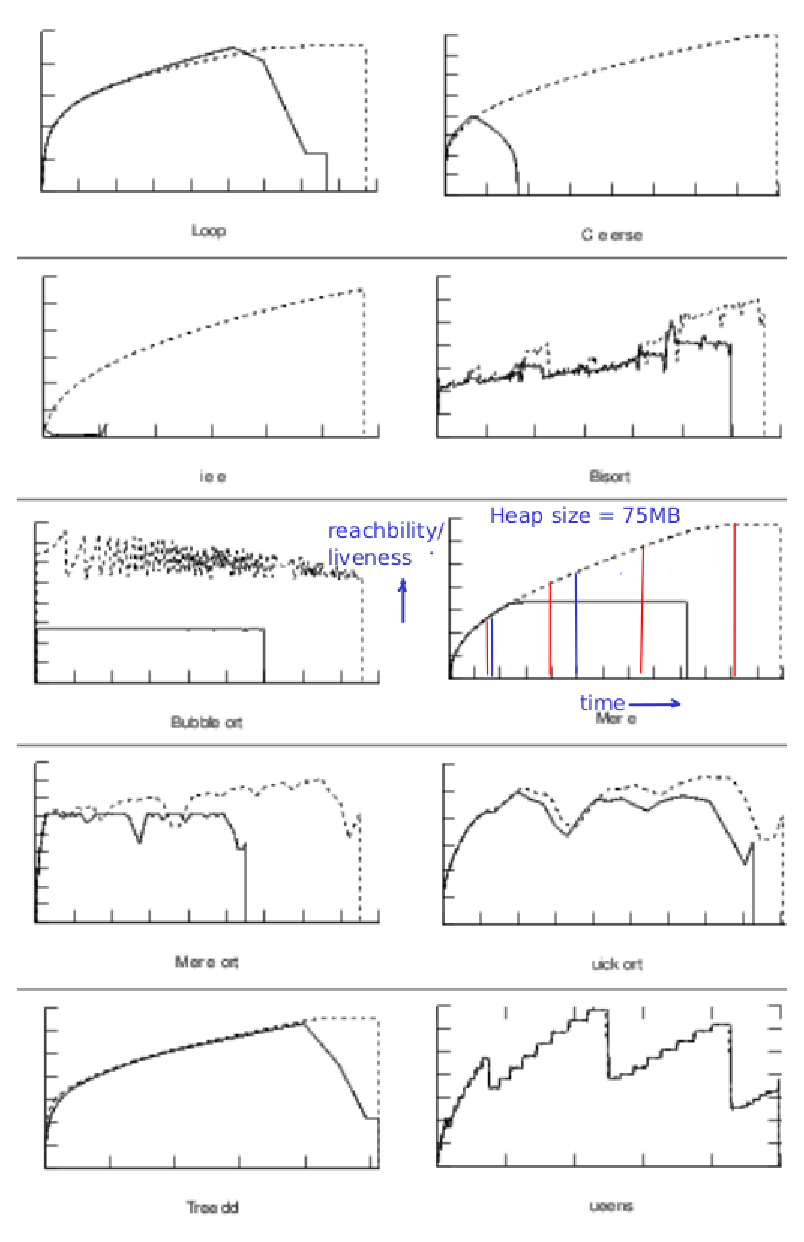
\epsfig{file=memory-usage.eps, width=12cm, height=15cm}}
%% \caption{Memory  usage of  programs. The  solid  lines represents
%%   number of  live cells and the  dashed lines show  the number of
%%   reachable cells.  The red and blue  lines represent invocations
%%   of RGC and  LGC---their heights indicate  the amount of memory
%%   copied.   {\color{red}{Caution:  Figures  are from  a  previous
%%       paper and are being used as placeholder}}}
%% \label{fig:memory-usage} \figrule
%% \end{figure}
%%\clearpage

\section{Related Work} Previous attempts to  increase  the space efficiency
of functional programs by additional  reclamation of memory fall in two
broad categories. In the first,  the program itself is instrumented to
manage  reclamation and reallocation  without the  aid of  the garbage
collector.    Such    attempts   include:   sharing    analysis   based
reallocation~\cite{jones89compile},                       deforestation
techniques~\cite{wadler88deforest,gill93ashort,chitil99deforest},   
methods  based  on   linear  logic~\cite{hofmann00linear}  and  region
analysis~\cite{tofte98region}.   Closer  to  our approach,  there  are
methods   that  enable   the   garbage  collector   to  collect   more
garbage~\cite{inoue88analysis,lee05static}   by
explicitly  nullifying  pointers  that  are not  live.   However,  the
nullification,  done   at  compile  time,   requires  sharing  (alias)
analysis.  Our  method, in contrast, does not  require sharing because
of the availability of the heap  itself at runtime.  To the best of our
knowledge, this is the first  attempt at liveness-based marking of the
heap during garbage collection.

\begin{figure}[t]
\centerline{\epsfig{file=lambda.eps, height=4cm, width=7cm}}
 \caption{Memory  usage and garbage collection pattern of  {\tt lambda}.} 
\label{fig:memory-usage-lambda} \figrule
\end{figure}

\section{Conclusions}
\label{sec:conclusion}
We have defined a notion of liveness on structured data;
this generalizes classical liveness and strong liveness.
We started with a general fully context-sensitive analysis which
we proved correct with respect to a minefield semantics
(this models the effect of garbage collection between every
evaluation step).

To avoid scalability issues (and to avoid performing part of
the liveness computation at run time)
we defined an 0-CFA version of this liveness analysis in which
demands for function $f$ at all calling contexts are conflated into 
a single demand $\sigma_f$.
This enabled us to treat the liveness equations symbolically obtaining
context-free grammars for liveness at each GC point (calls to user
functions and to $\CONS$).
These were then converted to DFAs for run-time consultation by the
garbage collector. Experiments confirm the precision of the analysis.

To obtain performance figures we compared a reachability-based garbage
collector with a liveness-based  collector.  This showed a decrease in
the  number  of  GCs,   more  garbage  collected  per  invocation.   A
significant benefit of LGC is  that programs can run in smaller memory
when compared to  RGC. This is potentially useful  in situations where
memory  is  limited---as with  embedded  systems.  For  a majority  of
programs, the garbage collection times were reduced.

One issue we  highlighted was that while fewer  nodes were marked (and
more garbage collected), sometimes  cons cells could be visited and
traversed  multiple times  with different  sets of  liveness  paths to
explore.  Further work includes  improvements to the classical copying
collector to reduce the cost of this.



\subsection*{Acknowledgements}
The authors  would like  to thank Hemanshu  Vadehra for  a preliminary
implementation of the prototype system. Amey Karkare was supported for
this work by the DST/SERC fast track scheme for young scientists.  

\bibliography{fun_hra}{}
\bibliographystyle{splncs}

\end{document}

%%%%%%%%%%%%%%%%%%%%%%%%%%%%%%%%%%%%%%%%%%%%%%%%%%%%%%%%%%%%%%%%%%%%%%%%%%%%%%%%%%%%%%%%%%%%%%%%%%%%%%%%%%%%%%%%%%%%%%%%%%%%%%%%%%%%%%%%%%%%%%%%%%%%%%%%%%%%%%%%%%%%%%%%%%%%%%%%%%%%%%%%%%%%%%%%%%%%%%%%%%%%%%%%%%%%%%%%%%%%%%%%%%%%%%%%%%%%%%%%%%%%%%%%%%%%%%%%%%%%%%%%%%%%%%%%%%%%%%%%%%%%%%%%%%%%%%%%%%%%%%%%%%%%%%%%%%%%%%%%%%%%%%%



\appendix
\section{Appendix stuff}

\paragraph{Safety of using the modified \CONS\  rule:}
Recall that while the correctness of the analysis was proved with
respect to  the $\len$ rules  in Figure~\ref{fig:live-judge}, the
equations   for  liveness   are  based   on  a   modification  of
$\mathit{ref}$    in    the    case    of   \CONS\  as  given    by
(\ref{eqn:mod-cons}).  We now show that  if the \bcar\,s and \bcdr\,s
in live access  paths resulting  from this  modification are
eliminated through  applications of $\hookrightarrow$,  we obtain
the same results as given by the original rules.


 
 
\comment{Proposal: We prove a result which goes as follows:

\begin{quote}
Lemma: Let  $\Lanv{i}{x}= \sigma$ for an a  program point $\pi_i$
and a variable  $x$, when the judgement is  based on the original
$\len$  rules.   Further, let  $\Lanv{i}{x}=  \sigma'$, when  the
judgement is based on $\len$ with the modified \CONS\ rule.  Then
$\sigma' \stackrel{*}{\hookrightarrow} \sigma$
\end{quote}

Here are some  ideas regarding how this can  be proved.  Consider
an arbitrary equation
$$ \Lanv{j}{y} = \ldots \Lanv{i}{x} \ldots$$ generated by the
analysis. 

Now assume that $\Lanv{i}{x}= \sigma$.   We want to find out what
happens to the access patterns in $\sigma$ in the access patterns
of \Lanv{j}{y}.   To answer this,  we put \# markers  around each
$\alpha \in \sigma$  and redo the equation using  an extension of
$\len$ to take  care of \#-tagged patterns.  We  can then observe
occurrences of \#-tagged patterns  in the liveness information at
$\pi_j$.

Here is  the $\len$ extension for  the original \CONS\  clause to take
care of the \#-tagged patterns:
$$\mathit{ref\/}((\CONS~x~y),\sigma,\Lfonly)
          = \{x.\#\alpha\# \mid \#\acar\alpha\# \in \sigma\} \cup
\{y.\#\alpha\# \mid \#\acdr\alpha\# \in \sigma\} $$
And here  is  the $\len$ extension for  the modified \CONS\  clause.
$$ \mathit{ref\/}((\CONS~x~y),\sigma,\Lfonly)
= \{x.\#\bcar\alpha\# \mid \#\alpha\# \in \sigma\} \cup
\{y.\#\bcdr\alpha\# \mid \#\alpha\# \in \sigma\} $$
All  other rules  remain unchanged.  Tracking a  pattern  through this
extension is sound because erasing the \#-tags would give us the same
liveness as the original rules. 

Let us also extend $\hookrightarrow$ to \#-tagged strings as:
$$\sigma_1  {\hookrightarrow} \sigma_2\,\, \mathit{iff}\,\, \sigma_2 =
\{\alpha_1 \#\alpha\# \alpha_2 \mid  \alpha_1 \#\alpha'\# \alpha2 \in
  \sigma_1\,\, and \,\, \{\alpha'\} \stackrel{*}{\hookrightarrow} \{\alpha\}\}$$
 
Now we have an  observation represented by the following diagram:

\centerline{\epsfig{file=diag1.eps, height=4cm}}

We need  to make this  observation general enough.   Therefore we
should prove  the observation even if \Lanv{i}{x}  = $\sigma$ had
patterns with \bcar\ and \bcdr.   We should be able to prove this
by structural induction on the rules.

How does  the observation prove  the original lemma?   Suppose we
replayed  judgements  with  ($\len$  +  \#) and  with  ($\len$  +
modified \CONS +  \#).  Suppose that $\pi_i$ is  the last program
point till which the results  are the same (because no \CONS\ was
encountered).  Now  consider a  $\sigma \in \Lanv{i}{x}$  for any
$x$.  Put \#-tags around each string in $\sigma$. Now we have the
diagram:

\centerline{\epsfig{file=diag2.eps, height=7cm}}


This shows that modulo erasure of \#-tags, using the original $\len$
judgement and  $\len$ judgement with modified \CONS\ rule followed by
$\hookrightarrow$ give the same liveness. 
   
And I would like  to conclude that it is all right  to do our analysis
with $\len$ + modified \CONS\ and then simplify using $\hookrightarrow$.

}

{\color{blue}\marginpar{From sec 3.1, liveness judgements}
\paragraph{Semantic considerations.}
The incremental liveness for generic primitive $\PRIM$ is given by
$\mathit{ref\/}((\PRIM~x~y),\sigma,\Lfonly) = 
           \{x.\epsilon,y.\epsilon\}$.
Earlier we suggested that classical strong liveness for addition,
but not division, could use the stronger
$ \{x.\epsilon,y.\epsilon \mid \epsilon \in \sigma\}$.
However this is invalid: garbage collection
could reuse dead, but reachable, $\CONS$ cell fields (of $v$ below)
thereby producing a stuck state in a dynamically typed language.
Hence we treat $+$ as like division not like addition---suppose
% $(FOO)$ is a user function which may cause garbage collection, and consider:
calling $\mbox{\footnotesize (FOO)}$ garbage collects and reallocates the cell pointed
to by `v' in:

\vspace{-15pt}

\begin{quote}
\footnotesize
\renewcommand{\arraystretch}{1}{
	  \begin{uprogram}
	  \UNL{1}  (\LET\ v\ $\leftarrow $\ (\CONS~2~3) \IN
	  \UNL{2}  (\LET\ w\ $\leftarrow $\ (FOO) \IN
	  \UNL{3}  (\LET\ x\ $\leftarrow $\ (\PRIM\ (\CAR\ v) 4) \IN
	  \UNL{4}  (\RETURN\ w))))
	\end{uprogram}}
\end{quote}
In principle, {\em dead code removal} of
$(\PRIM\ (\CAR\ {\rm v})\ 4)$
would render the stronger version valid, but still requires static typing
to avoid the risk of {\em removing} a stuck state.
We restrict ourselves to liveness annotation rather than code transformation.
}

%%%%%%%%%%%%%%%%%%%%%%%%%%%%%%%%%%%%%%%%%%%%%%%%%%%%%%%%%%%%%%%
\begin{figure}[t]
\footnotesize
Old version of the liveness rules...

\infrule[ret-live]
        {}
        {(\RETURN~x),\sigma,\Lfonly \len  x.\sigma}
%%%%%%%%%%%%%%%%%%%%%%%%%%%%%%%%%%%%%%%%%%%%%%%%%%%%%%%%%%%%%%%
\infrule[if-live]
        { e_1, \sigma,\Lfonly \len \Lv_1
          \andalso e_2, \sigma,\Lfonly \len  \Lv_2}
        {(\SIF~x~e_1~e_2),\sigma,\Lfonly \len
               \Lv_1\cup\Lv_2\cup \{x.\epsilon\}}
%%%%%%%%%%%%%%%%%%%%%%%%%%%%%%%%%%%%%%%%%%%%%%%%%%%%%%%%%%%%%%%
\infrule[let-live]
        {e, \sigma,\Lfonly  \len  \Lv}
        {(\LET~x \leftarrow  s~\IN~e),
          \sigma,\Lfonly \len   \Lv\setminus \{x.*\} \cup
          \mathit{ref\/}(s,\Lv(x),\Lfonly)}

%%%%%%%%%%%%%%%%%%%%%%%%%%%%%%%%%%%%%%%%%%%%%%%%%%%%%%%%%%%%%%%

\infrule[live-define]
        {e_f, \sigma, \Lfonly  \len
%            \bigcup \{z_i.\Lf{f}{i}{\sigma} \mid i=1,\ldots, n\}
           \bigcup_{i=1}^n y_i.\Lf{f}{i}{\sigma}
              \mbox{ for each $f$ and $\sigma$}
        }
        { d_1 \ldots d_k \fen \Lfonly
\\ \mbox{where }
     (\DEFINE\ (f\ z_1\ \ldots\ z_n)\ \ \ e_f) \mbox{ is a member of }
        d_1 \ldots d_k}
\figrule
  \caption{Liveness Judgement Rules}\label{fig:live-judge-old}
\normalsize
\end{figure}


%%%%%%%%%%%%%%%%%%%%%%%%%%%%%%%%%%%%%%%%%%%%%%%%%%%%%%%% 

  \newgray{lightgray}{.75}
%\newcommand{\dem}[1]{\red{\scriptsize{$#1$}}}
\newcommand{\dem}[1]{\psframebox[linestyle=none,fillstyle=none,fillcolor=lightgray]{\rule[-1pt]{0pt}{8pt}{\scriptsize $#1$}}\hspace*{1pt}}
%\newcommand{\liv}[1]{\blue{\scriptsize{$#1$}}}
\newcommand{\liv}[1]{\psframebox[linestyle=none,fillstyle=solid,fillcolor=lightgray]{\rule[-1pt]{0pt}{8pt}{\scriptsize $#1$}}\hspace*{1pt}}

%%%%%%%%%%%%%%%%%%%%%%%%%%%%%%%%%%%%%%%%%%%%%%%%%%%%%%%% 



\begin{figure}[h!]
\psset{unit=1mm,nodesep=1mm,labelsep=0.5mm,arrows=->,linewidth=.1,framesep=0.2mm}
\begin{center}
  \begin{pspicture}(0,0)(120,50)
%\psgrid[xunit=1cm,yunit=1cm,gridwidth=.2pt,subgridwidth=.1pt,subgriddiv=5,subgridcolor=gray,gridcolor=blue](0,0)(12,5)
 \footnotesize
   \putnode{let1}{origin}{15}{50}{$\pi_1$:\LET}

    \putnode{test1}{let1}{-12}{-7}{\xtest}
    \putnode{null}{let1}{0}{-7}{$\pi_2$:\NULLQ}
    \putnode{lista1}{null}{0}{-7}{$\pi_3$:\lista}
    \putnode{if}{let1}{18}{-7}{$\pi_4$:\SIF}

    \putnode{test2}{if}{-8}{-7}{$\pi_5$:\xtest}
    \putnode{listb1}{if}{3}{-7}{$\pi_6$:\listb}
    \putnode{let2}{if}{14}{-7}{$\pi_7$:\LET}

    \putnode{tl1}{let2}{-22}{-7}{\xtl}
    \putnode{cdr}{let2}{-5}{-7}{$\pi_8$:\CDR}
    \putnode{lista2}{cdr}{0}{-7}{$\pi_9$:\lista}
    \putnode{let3}{let2}{15}{-7}{$\pi_{10}$:\LET}


\putnode{rec1}{let3}{-13}{-7}{\xrec}
\putnode{append}{let3}{0}{-7}{$\pi_{11}$:\append}
\putnode{tl2}{append}{-10}{-7}{$\pi_{12}$:\xtl}
\putnode{listb2}{append}{5}{-7}{$\pi_{13}$:\listb}

\putnode{let4}{let3}{17}{-7}{$\pi_{14}$:\LET}
\putnode{hd1}{let4}{-5}{-7}{\xhd}
\putnode{car}{let4}{4}{-7}{$\pi_{15}$:\CAR}
\putnode{lista3}{car}{0}{-7}{$\pi_{16}$:\lista}

\putnode{let5}{let4}{16}{-7}{$\pi_{17}$:\LET}


\putnode{ans1}{let5}{-4}{-7}{\xans}
\putnode{cons}{let5}{6}{-7}{$\pi_{18}$:\CONS}
\putnode{hd2}{cons}{-10}{-7}{$\pi_{19}$:\xhd}
\putnode{rec2}{cons}{10}{-7}{$\pi_{20}$:\xrec}
\putnode{ans2}{let5}{19}{-7}{$\pi_{21}$:\xans}
%%%%%%%%%%%%%%%%%%%%%%%%%%%%%%%%%%%%%%%%%%%%%%%%%%%%%%%%%%%%%%5

%% \putnode{x}{let1}{0}{3}{\dem{\sigma}}
%% \putnode{x}{if}{0}{3}{\dem{\sigma}}
%% \putnode{x}{let2}{0}{3}{\dem{\sigma}}
%% \putnode{x}{let2}{-7}{0}{\liv{\Lv_4}}
%% \putnode{x}{let3}{0}{3}{\dem{\sigma}}
%% \putnode{x}{let4}{0}{3}{\dem{\sigma}}
%% \putnode{x}{ans2}{0}{3}{\dem{\sigma}}
%% \putnode{x}{ans2}{-8}{0}{\liv{\Lv_1}}
%% %\putnode{x}{ans2}{9}{0}{\liv{\Lv_0}}
%% \putnode{x}{plus}{0}{3}{\dem{\sigma}}
%% \putnode{x}{rec2}{1}{4}{\dem{\epsilonset}}
%% \putnode{x}{plus}{-7}{0}{\liv{\Lv_6}}
%% %\putnode{x}{let4}{-7}{0}{\liv{\{\xrec\}}}
%% \putnode{x}{len}{3}{3}{\dem{\epsilonset}}
%% \putnode{x}{len}{-7}{0}{\liv{\Lv_3}}
%% \putnode{x}{tl2}{0}{4}{\dem{\Lf{\xlen}{1}(\epsilonset)}}
%% \putnode{x}{tl2}{-6}{0}{\liv{\Lv_3}}
%% %\putnode{x}{let3}{-10}{0}{\liv{\xtl.\Lf{\xlen}{1}(\epsilonset)}}
%% \putnode{x}{cdr}{0}{4}{\dem{\Lf{\xlen}{1}(\epsilonset)}}
%% \putnode{x}{cdr}{-7}{0}{\liv{\Lv_4}}
%% \putnode{x}{l2}{0}{4}{\dem{\epsilonset \cup \acdr\Lf{\xlen}{1}(\epsilonset)}}
%% \putnode{x}{l2}{-5}{0}{\liv{\Lv_4}}
%% \putnode{x}{zero}{0}{3}{\dem{\sigma}}
%% \putnode{x}{zero}{-3}{0}{\liv{\Lv_0}}
%% \putnode{x}{test2}{0}{3}{\dem{\epsilonset}}
%% \putnode{x}{test2}{-7}{0}{\liv{\Lv_5}}
%% \putnode{x}{if}{-6}{0}{\liv{\Lv_3}}
%% \putnode{x}{null}{0}{3}{\dem{\epsilonset}}
%% \putnode{x}{null}{-9}{0}{\liv{\Lv_4}}
%% \putnode{x}{l1}{0}{3}{\dem{\epsilonset}}
%% \putnode{x}{vone2}{0}{3}{\dem{\epsilonset}}
%% \putnode{x}{one}{0}{3}{\dem{\epsilonset}}
%% \putnode{x}{let5}{0}{3}{\dem{\sigma}}
%% \putnode{x}{l1}{-5}{0}{\liv{\Lv_4}}
%% %\putnode{x}{let1}{-17}{-1}{\liv{\{\xl\} \cup \xl.\acdr\Lf{\xlen}{1}(\epsilonset)}}
%% \putnode{x}{let1}{8}{0}{\liv{\Lv_0}}
%% \putnode{x}{let1}{-7}{0}{\liv{\Lv_4}}
%% %\putnode{x}{if}{7}{0}{\liv{\Lv_0}}
%% %\putnode{x}{let2}{8}{0}{\liv{\Lv_0}}
%% %\putnode{x}{let3}{8}{0}{\liv{\Lv_0}}
%% \putnode{x}{let3}{-7}{0}{\liv{\Lv_3}}
%% %\putnode{x}{let4}{9}{0}{\liv{\Lv_0}}
%% \putnode{x}{let4}{-7}{0}{\liv{\Lv_2}}
%% \putnode{x}{vone2}{-8}{0}{\liv{\Lv_6}}
%% \putnode{x}{rec2}{-8}{0}{\liv{\Lv_6}}
%% \putnode{x}{let5}{-8}{0}{\liv{\Lv_6}}
%% \putnode{x}{one}{-6}{0}{\liv{\Lv_2}}
\ncline{-}{let1}{test1}
\ncline{-}{let1}{null}
\ncline{-}{let1}{if}
\ncline{-}{null}{lista1}

\ncline{-}{if}{test2}
\ncline{-}{if}{listb1}
\ncline{-}{if}{let2}
\ncline{-}{let2}{tl1}
\ncline{-}{let2}{cdr}
\ncline{-}{let2}{let3}
\ncline{-}{cdr}{lista2}

\ncline{-}{let3}{rec1}
\ncline{-}{let3}{append}
\ncline{-}{let3}{let4}

\ncline{-}{append}{tl2}
\ncline{-}{append}{listb2}

\ncline{-}{let4}{let5}
\ncline{-}{let4}{hd1}
\ncline{-}{let4}{car}
\ncline{-}{car}{lista3}
%% \ncline{-}{len4}{tl2}
%% \ncline{-}{let4}{vone1}
%% \ncline{-}{let4}{one}
%% \ncline{-}{let4}{let5}
\ncline{-}{let5}{ans1}
\ncline{-}{let5}{cons}
\ncline{-}{cons}{hd2}
\ncline{-}{cons}{rec2}
%% \ncline{-}{let5}{plus}
\ncline{-}{let5}{ans2}
\end{pspicture}
 \end{center}

  \caption{Example to illustrate liveness computation}\label{fig:live-examp}
\figrule
\normalsize
\end{figure}


\newpage



\begin{figure}[t]
  \begin{tabularx}{320pt}{|| c | X | X | X ||}
\hline
Pgm  Pt & Demand  & Pre & Post \\
\hline 
$\pi_1$ & $\sigma$ & \{\lista\} $\cup$ \listb.$\sigma$ $\cup$ \lista.\{\acdr\}\Lf{\append}{1}(\{\bcdr\}$\sigma$)  $\cup$ \lista.\{\acar\bcar\}$\sigma$ $\cup$ \listb.\Lf{\append}{2}(\{\bcdr\}$\sigma$) & $\phi$ \\
\hline
%% $\pi_2$ & $\epsilonset$ & \{\lista\} $\cup$ \listb.$\sigma$  $\cup$ \lista.\{\acdr\}\Lf{\append}{1}(\{\bcdr\}$\sigma$)  $\cup$ \lista.\{\acar\bcar\}$\sigma$ $\cup$ \listb.\Lf{\append}{2}(\{\bcdr\}$\sigma$) & \listb.$\sigma$ $\cup$ \{\lista\}  $\cup$ \lista.\{\acdr\}\Lf{\append}{1}(\{\bcdr\}$\sigma$)  $\cup$ \lista.\{\acar\bcar\}$\sigma$ $\cup$ \listb.\Lf{\append}{2}(\{\bcdr\}$\sigma$) \\
%% \hline
$\pi_3$ & $\epsilonset$ &\{\lista\} $\cup$ \listb.$\sigma$  $\cup$ \lista.\{\acdr\}\Lf{\append}{1}(\{\bcdr\}$\sigma$)  $\cup$ \lista.\{\acar\bcar\}$\sigma$ $\cup$ \listb.\Lf{\append}{2}(\{\bcdr\}$\sigma$)  & \listb.$\sigma$ $\cup$ \{\lista\}  $\cup$ \lista.\{\acdr\}\Lf{\append}{1}(\{\bcdr\}$\sigma$)  $\cup$ \lista.\{\acar\bcar\}$\sigma$ $\cup$ \listb.\Lf{\append}{2}(\{\bcdr\}$\sigma$) \\
\hline
%%%%%%%%%%%%%%%%%%%%%%%%%%%%%%%%%%%%%%%%%%%%%%%%%%%%%%%%%%%%%%%%%%%%
%% $\pi_4$ & $\sigma$ &\{\xtest\} $\cup$ \listb.$\sigma$ $\cup$ \{\lista\}  $\cup$ \lista.\{\acdr\}\Lf{\append}{1}(\{\bcdr\}$\sigma$)  $\cup$ \lista.\{\acar\bcar\}$\sigma$ $\cup$ \listb.\Lf{\append}{2}(\{\bcdr\}$\sigma$)  & $\phi$ \\
%% \hline
%% $\pi_5$ & \epsilonset & \{\xtest\} $\cup$ \listb.$\sigma$ $\cup$ \{\lista\}  $\cup$ \lista.\{\acdr\}\Lf{\append}{1}(\{\bcdr\}$\sigma$)  $\cup$ \lista.\{\acar\bcar\}$\sigma$ $\cup$ \listb.\Lf{\append}{2}(\{\bcdr\}$\sigma$)   & \listb.$\sigma$ $\cup$ \{\lista\}  $\cup$ \lista.\{\acdr\}\Lf{\append}{1}(\{\bcdr\}$\sigma$)  $\cup$ \lista.\{\acar\bcar\}$\sigma$ $\cup$ \listb.\Lf{\append}{2}(\{\bcdr\}$\sigma$)  \\
%% \hline
%% $\pi_6$ & $\sigma$ & \listb.$\sigma$ & $\phi$ \\
%% \hline
%% %%%%%%%%%%%%%%%%%%%%%%%%%%%%%%%%%%%%%%%%%%%%%%%%%%%%%%%%%%%%%%%%%%%%
%% $\pi_7$ & $\sigma$  & \{\lista\}  $\cup$ \lista.\{\acdr\}\Lf{\append}{1}(\{\bcdr\}$\sigma$)  $\cup$ \lista.\{\acar\bcar\}$\sigma$ $\cup$ \listb.\Lf{\append}{2}(\{\bcdr\}$\sigma$)  & $\phi$\\
%% \hline
%% $\pi_8$ & \Lf{\append}{1}(\{\bcdr\}$\sigma$) & \{\lista\}  $\cup$ \lista.\{\acdr\}\Lf{\append}{1}(\{\bcdr\}$\sigma$)  $\cup$ \lista.\{\acar\bcar\}$\sigma$ $\cup$ \listb.\Lf{\append}{2}(\{\bcdr\}$\sigma$)   & \{\lista\} $\cup$ \lista.\{\acar\bcar\}$\sigma$ $\cup$ \listb.\Lf{\append}{2}(\{\bcdr\}$\sigma$) \\
%% \hline
$\pi_9$ & \epsilonset $\cup$ \{\acdr\}\Lf{\append}{1}(\{\bcdr\}$\sigma$)  & \{\lista\}  $\cup$ \lista.\{\acdr\}\Lf{\append}{1}(\{\bcdr\}$\sigma$)  $\cup$ \lista.\{\acar\bcar\}$\sigma$ $\cup$ \listb.\Lf{\append}{2}(\{\bcdr\}$\sigma$)   & \{\lista\} $\cup$ \lista.\{\acar\bcar\}$\sigma$ $\cup$ \listb.\Lf{\append}{2}(\{\bcdr\}$\sigma$) \\
\hline
%%%%%%%%%%%%%%%%%%%%%%%%%%%%%%%%%%%%%%%%%%%%%%%%%%%%%%%%%%%%%%%%%%%%
%% $\pi_{10}$ &$\sigma$ & \{\lista\}  $\cup$ \lista.\{\acar\bcar\}$\sigma$ $\cup$ \xtl.\Lf{\append}{1}(\{\bcdr\}$\sigma$) $\cup$  \listb.\Lf{\append}{2}(\{\bcdr\}$\sigma$)  & $\phi$ \\
%% \hline
$\pi_{11}$ & \{\bcdr\}$\sigma$ & \{\lista\}  $\cup$ \lista.\{\acar\bcar\}$\sigma$ $\cup$ \xtl.\Lf{\append}{1}(\{\bcdr\}$\sigma$) $\cup$  \listb.\Lf{\append}{2}(\{\bcdr\}$\sigma$) & \lista $\cup$ \lista.\{\acar\bcar\} \\
\hline
$\pi_{12}$ &\Lf{\append}{1}(\{\bcdr\}$\sigma$)   &\{\lista\}  $\cup$ \lista.\{\acar\bcar\}$\sigma$ $\cup$ \xtl.\Lf{\append}{1}(\{\bcdr\}$\sigma$) $\cup$  \listb.\Lf{\append}{2}(\{\bcdr\}$\sigma$)  &  \\
\hline
$\pi_{13}$ & \Lf{\append}{2}(\{\bcdr\}$\sigma$)  &\{\lista\}  $\cup$ \lista.\{\acar\bcar\}$\sigma$ $\cup$ \xtl.\Lf{\append}{1}(\{\bcdr\}$\sigma$) $\cup$  \listb.\Lf{\append}{2}(\{\bcdr\}$\sigma$)  &  \\
\hline
%%%%%%%%%%%%%%%%%%%%%%%%%%%%%%%%%%%%%%%%%%%%%%%%%%%%%%%%%%%%%%%%%
$\pi_{14}$ & $\sigma$ & \{\lista\} $\cup$ \lista.\{\acar\bcar\}$\sigma$ $\cup$ \xrec.\{\bcdr\}$\sigma$ & $\phi$ \\
\hline
%% $\pi_{15}$ & \{\bcar\}$\sigma$  & \{\lista\} $\cup$ \lista.\{\acar\bcar\}$\sigma$ $\cup$ \xrec.\{\bcdr\}$\sigma$   &  \xrec.\{\bcdr\}$\sigma$\\
%% \hline
%% $\pi_{16}$ & \epsilonset $\cup$ \{\acar\bcar\}$\sigma$ & \{\lista\} $\cup$ \lista.\{\acar\bcar\}$\sigma$ $\cup$ \xrec.\{\bcdr\}$\sigma$  & \xrec.\{\bcdr\}$\sigma$ \\
%% \hline
$\pi_{17}$ & $\sigma$ & \xhd.\{\bcar\}$\sigma$ $\cup$ \xrec.\{\bcdr\}$\sigma$   & $\phi$  \\
\hline
%%%%%%%%%%%%%%%%%%%%%%%%%%%%%%%%%%%%%%%%%%%%%%%%%%%%%%%%%%%%%%%%%%%
$\pi_{18}$ & $\sigma$ & \xhd.\{\bcar\}$\sigma$ $\cup$ \xrec.\{\bcdr\}$\sigma$ & $\phi$  \\
\hline
$\pi_{19}$ &  \{\bcar\}$\sigma$        & \xhd.\{\bcar\}$\sigma$ $\cup$ \xrec.\{\bcdr\}$\sigma$ &   \\
\hline
$\pi_{20}$ &   \{\bcdr\}$\sigma$       & \xhd.\{\bcar\}$\sigma$ $\cup$ \xrec.\{\bcdr\}$\sigma$ &   \\
\hline
$\pi_{21}$ & $\sigma$ & \xans.$\sigma$ & $\phi$  \\
\hline
\end{tabularx}
  \caption{Liveness annotations for the body of \append}\label{fig:xe_append}
\figrule
\normalsize
\end{figure}
